\documentclass[fleqn]{report}
\usepackage{remhref}
\usepackage{nowidow}

\begin{document}

\title{Course Notes for Linear Algebra}
\author{Remkes Kooistra \\
	The King's University}
\date{\today}
\maketitle

\setcounter{tocdepth}{0}
\tableofcontents
\numberwithin{thm}{section}

\renewcommand{\chaptername}{Lecture}
\renewcommand{\abstractname}{License}

\begin{abstract}
This work is licensed under the Creative Commons
Attribution-ShareAlike 4.0 International License.
\end{abstract}

\chapter*{Welcome to the Course}
\label{welcome}

This courses uses a pedagogical model known either as blended
learning or the flipped classroom. In this model, the majority of the
content will be delivered outside of class time through
two avenues: these notes and a series of short videos.
You will be required to watch one of the short videos 
before most class periods. We will
begin each lecture period assuming you have watched the
required video.

The videos are used to introduce the main ideas of the
course. They are the explanation. Matched with each video 
will be a short section of notes. The
notes are provided for reference, so that after you've watched
the video, you can use the notes to remind yourself of the
content and refer to useful ideas, concepts and formulae. The
notes are not primarily written to explain the material;
instead, they are written to provide a record of the ideas in
the video for your reference. The notes are light on
examples. The lecture time will be mostly devoted to
necessary practice and examples.

The course is organized into twenty-two lectures; the videos
and the activities are numbered to match these lectures. There
is a detailed schedule on the course website showing when the
various lectures happen over the term. Please use this
schedule to ensure you watch the appropriate videos before
class and bring the appropriate sections of the notes. 

\section*{Other Resources}

In addition to the notes associated to each lecture, there are
a number of other resources which are distributed via
the course website. These resources have been developed to
assist you, so please make use of them. 

\begin{itemize}
\item A complete formula sheet. All of the basic formulas and
rules for calculation are included on this sheet. There are
sections on algebra, trigonometry, derivatives and integrals.
Later in the document are some pieces of linear algebra
reference as well.
\item A notation reference. This reference covers a number of
notations used in the course which may be unfamiliar. 
\item A course outcomes sheet. This was originally
developed as a study aid for students. It summarizes the main
definitions and concepts of the course, as well as the types
of questions your will encounter on assignments and exams. In
particular, it gives a guide to the material on the exam. If
you want to know whether a definition, topic or type of
problem might show up on the exam, consult this sheet. 
\end{itemize}

\section*{Perspectives and Philosophy}

In addition to the strictly mathematical material of the
course, I will try to share some ideas which give perspective
and context to mathematics. This include the philosophy of
mathematics, the aesthetics of mathematics, and how our own worldview and
assumptions influence mathematical thought. Linear algebra is
perhaps the most abstract mathematical course offered at
King's; at least, it offers the most oppotunity for
abstract thinking. Therefore, I use this course as a venue for
talking about abstraction in the context of perspectives and
philosophy.

\chapter{Themes of the Course}
\label{themes}

\section{Algebra}

Linear \emph{algebra} is, as expected, an algebra course. (It
is the only strictly algebra course taught at King's, though
elsewhere, it would be the first of a sequence of algebra
courses.)

The word `algebra' does not mean the same thing in university
mathematics as it did in high-school mathematics. Previously,
the world `algebra' usually signaled the use of variables:
$3+5 = 8$ is arithmetic, but $3 + x = 8 \implies x = 5$ is
algebra. From that point, algebra became the manipulation of
equations (and inequalities) with variables, particularly
focusing on solving polynomials and rational functions.

In academic mathematics, algebra has a much broader and deeper
sense. It is a whole branch of mathematics, with many
subdisciplines: linear algebra, abstract algebra, homological
algebra, etc. One of the goals of this course will be to build
as sense of what we mean by the term `algebra'. I'll give a
definition right now, at the start, but it's a difficult
definition to understand; hopefully the course will provide
the necessary elaboration.

\begin{defn}
\emph{Algebra} is the study of sets with structure. It
investigates possible structures on sets, the rules obeyed by
those structures, and the interaction of various structures. 
\end{defn}

\section{Abstraction}

The definition of algebra just stated is an immensely
abstract definition. I haven't specified what sets or what
structures I'm talking about. (I could say that we are looking
at \emph{algebraic structures}, but that doesn't actually add
any insight; it just delays the question.) The definition is
very broad, applies to a huge variety of sets and structures.
Abstraction is built into the very nature of algebra. 

In the calculus courses, I often motivate the material by its
applications. (The two most often used motivations are the
Newtonian physics and percentage growth in ecology or
finance.) In this sense, I'm treating the calculus as applied
mathematics: mathematics driven by and designed for the
solving of certain extra-mathematical problems. This is a
reasonable approach for calculus, both for historical and
pedagogical reasons. 

In this course, there will be points where I emphasize the
practical applications of linear algebra, of which there are
many. However, my primary motivation for the course will be
intrinsic and abstract: I want to study sets and their
structure simply for the mathematical joy of it. This is the
one course at King's which is most suited to presenting the
goals and ideas of abstract mathematics, in and of themselves. 

\section{Geometry}

Though the subjet is called `algebra', linear algebra is a
very geometric discpline. Given my background as a geometer,
my approach to the course will be heavily geometric. We
will start with vectors, which is a geometric discpline,
though it has rich algebraic structre. Throughout the course,
we will play the geometry and algebra against each other and
use each to understand the other better. This interplay drives
the discpline. In many ways, this will be a geomety course
hiding under the title of an algebra course.

In addition, we will not restrict ourselves for conventional
two and three dimensional geometry. The definitions of this
course are very general, so we will try to do geometry in any
(finite) dimension. A major challenge of the course is going
from familiar, visible three dimensions to un-visualizable
higher dimensional geometry.

\section{Flatness}

While a geometry course, the geometry we are considering will
be very restricted. The `linear' in linear algebra refers to
lines, so we will start with the geometry of lines. However,
the important property of a line, in our context, is the fact
that it is straight: it doesn't curve. Linear algebra is the
geomtery of flat things.

Therefore, curved, bent and broken objects are off limits. We
will investigate the geometry of flat objects: points, lines,
planes and higher dimensional analogue. A great advantage of
this restriction is the fact that flat things are very
accessable. The geometry of curved objects is an immensely
complicated and difficult subject. By restricting to flat
objects, we can produce a wide range of accessible
mathematical results. 

\section{Symmetry}

Other than flatness, our other major geometric theme is
symmetry. Many of the definitions and propositions produced in
this course can be stated in terms of some kind of symmetry.
Speaking broadly, I want to thing of symmetry as preservation:
the symmetry of a shape is some kind of operation which keeps
the shape intact, preserves it. Throughout linear algebra, we
will be talking about the preservation of various kinds of
shapes and flat objects.

With the interplay between algebra and geometry mentioned
above, we will also translate this idea of symmetry back to
algebra to give a understanding of algebraic symmetry. 

\section{Proof}

Proofs are another major difference between the grade-school
understanding of algebra and the academic sense of the word.
Algebra is originally introduced to solve problems involving
unknown quantities, usually by solving equations. Algebra is a
problem-solving technique. In academic mathematics, we are
usually more concerned with conjectures about mathematical
objects and the proofs of those conjecture. In this course,
we'll introduce the idea of conjectures, propositions,
theorems and proofs. We'll do a small amount of proving on the
assignments to build a flavour for proof-based mathematics.

\chapter{Vectors}
\label{Vectors}

\section{Definitions}

\begin{defn}
In linear algebra, ordinary numbers (intergers, rational
numbers or real numbers) are called \emph{scalars}.
\end{defn}

\begin{defn}
A \emph{vector} is a finite ordered list of scalars. Vectors
can be written either as columns or rows. 
If a vector is a list of the numbers $4$, $15$, $\pi$ and $-e$ (in that
order), we write the vector in one of two ways.
\begin{displaymath}
\colvec{4}{4}{15}{\pi}{e} \hspace{1cm} \text{ or }
\hspace{1cm} (4, 15, \pi, -e)
\end{displaymath}
\end{defn}

In these notes, we will exclusively use column vectors.

\begin{defn}
Let $n$ be a positive integer. \emph{Real Euclidean Space} or
\emph{Cartesian Space}, written $\RR^n$, is the set of all
vectors of length $n$ with real number entries. An arbitrary
element of $\RR^n$ is written as a column. 
\begin{displaymath}
\colvec{4}{x_1}{x_2}{\vdots}{x_n}
\end{displaymath}
We say that $\RR^n$ has \emph{dimension} $n$. 
\end{defn}

\begin{defn}
The scalars $x_i$ in a vector are
called the \emph{entries}, \emph{coordinates} or \emph{components} of that
vector. Specifically, $x_1$ is the first coordinate, $x_2$ is
the second coordinate, and so on. 
For $\RR^2$, $\RR^3$ and $\RR^4$, we use the letters $w,x,y,z$
instead of $x_i$.
\begin{displaymath}
\colvec{2}{x}{y} \in \RR^2 \hspace{1cm}
\colvec{3}{x}{y}{z} \in \RR^3 \hspace{1cm}
\colvec{4}{w}{x}{y}{z} \in \RR^4
\end{displaymath}
\end{defn}

\begin{defn}
In any $\RR^n$, the \emph{origin} is the unique point given by a
vector of zeros. It is also called the zero vector. It is
considered the centre point of Cartesian space.
\begin{displaymath}
\colvec{4}{0}{0}{\vdots}{0}
\end{displaymath}
\end{defn}

\begin{figure}[t]
\centering

\includegraphics[width=8cm]{figure1.eps}
\caption{Points in the Cartesian Plane $\RR^2$}
\label{Points in the Cartesian Plane}
\end{figure}

Cartesian space, particularly the Cartesian plane, is a familiar
object from high-school mathematics. We usually visualize
Cartesian space by drawing axes, one in each
independent perpendicular direction. 
In this visualization, the vector
\scalebox{0.7}{$\colvec{2}{a}{b}$} corresponds to the
unique point we get moving $a$ units in the direction of the $x$
axis and $b$ units in the direction of the $y$ axis.
Figure \ref{Points in the Cartesian Plane} shows the location
of several points in $\RR^2$.

\begin{figure}[t]
\centering
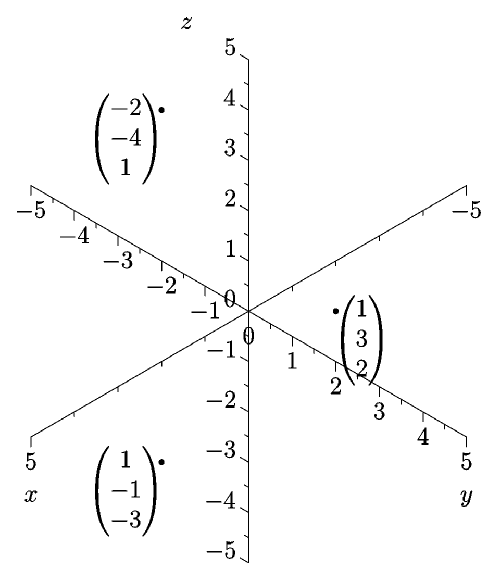
\includegraphics[width=7cm]{figure2.eps}
\caption{Points in Cartesian three-space $\RR^3$}
\label{Points in Cartesian three-space}
\end{figure}

As with $\RR^2$, the point
\scalebox{0.7}{$\colvec{3}{a}{b}{c}$} $\in \RR^3$ is the
unique point we find by moving $a$ units in the $x$ direction,
$b$ units in the $y$ direction and $c$ units in the $z$
direction. When we visualize $\RR^2$, we conventionally write
the $x$ axis horizontally, with a positive direction to the
right, and the $y$ axis vertically, with a positive direction
upwards. For $\RR^3$, the $x$ and $y$ axes form a flat plane
and the $z$ axis extend vertically from that plan, as shown in
Figure \ref{Points in Cartesian three-space}. Notice, in both
cases, we needed to choose directions for the axes.

\begin{defn}
A choice of axis directions in a visualization of $\RR^n$ 
is called an \emph{orientation}.
\end{defn}

While we can visualize $\RR^2$ and $\RR^3$ relatively easily and
efficiently, but we can't visualize any higher $\RR^n$. However,
this doesn't prevent us from working in higher dimensions. We need to
rely on the algebraic descriptions of vectors instead of the
drawings and visualizations of $\RR^2$ and $\RR^3$. 

In our visualizations of $\RR^2$ and
$\RR^3$, we see the different axes as fundementally
different perpendicular directions. We can think of $\RR^2$ as
the space with two independent directions and $\RR^3$ as the
space with three independent directions. Similarly, $\RR^4$ is
the space with four perpendicular, independent directions, even
though it is impossible to visualize such a thing. 
Likewise, $\RR^n$ is the space with $n$ independent directions. 

\begin{figure}[t]
\centering

\includegraphics[width=8cm]{figure3.eps}
\caption{Vectors as Points and Directions}
\label{Points and Directions}
\end{figure}

\section{Points or Directions?}

We can think of a element of $\RR^2$, say
\scalebox{0.7}{$\colvec{2}{1}{4}$}, as both the point located
at \scalebox{0.7}{$\colvec{2}{1}{4}$} and the vector drawn
from the origin to the point
\scalebox{0.7}{$\colvec{2}{1}{4}$}, as shown in Figure
\ref{Points and Directions}. Though these two ideas are
distinct, we will frequently change perspective between them.
Part of becoming proficient in vector geometry is becoming
accustomed to the switch between the perspectives of points
and directions.

\section{Linear Operations}

The environment for linear algebra is $\RR^n$. Algebra is
concerned with operations on sets, so we want to know what
operations we can perform on $\RR^n$. There are several.

\begin{figure}[t]
\centering
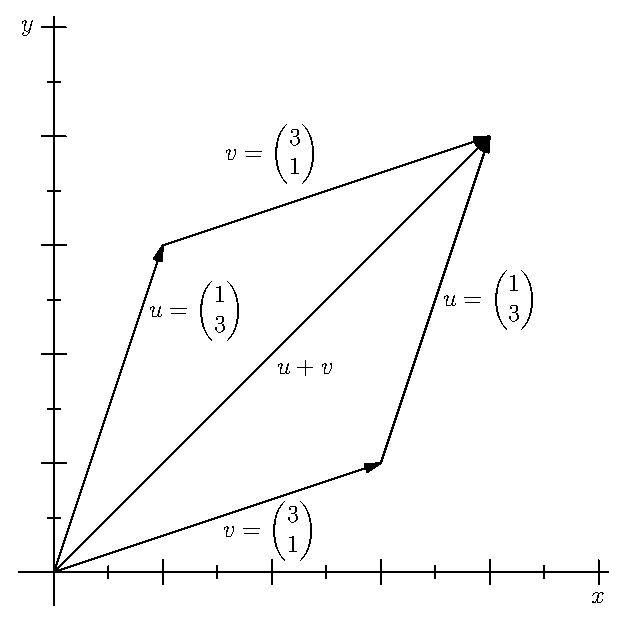
\includegraphics[width=8cm]{figure4.eps}
\caption{Visualizing Vector Addition}
\label{Visualizing Vector Addition}
\end{figure}

\begin{defn}
The \emph{sum} of two vectors $u$ and $v$ in $\RR^n$ is the
sum taken componentwise. 
\begin{equation*}
u + v = \colvec{4}{u_1}{u_2}{\vdots}{u_n} +
\colvec{4}{v_1}{v_2}{\vdots}{v_n} = \colvec{4}{u_1 + v_1}{u_2
+ v_2}{\vdots}{u_n + v_n}
\end{equation*}
\end{defn}

The sum is visuzliazed by placing the start of the second
vector at the end of the first, as in Figure \ref{Visualizing
Vector Addition}. Note that we can only add two vectors in
the same dimension. We can't add a vector in $\RR^2$ to a
vector in $\RR^3$.

\begin{figure}[t]
\centering

\includegraphics[width=8cm]{figure5.eps}
\caption{Visualizing Scalar Multiplication}
\label{Visualizing Scalar Multiplication}
\end{figure}

\begin{defn}
If $u$ is a vector in $\RR^n$ and $a \in
\RR$ is a real number, then the \emph{scalar multiplication} of
$u$ and $a$ is multiplication by $a$ in each component of $u$.
By convention, scalar multiplication is written with the
scalar on the left of the vector.
\begin{equation*}
au = a \colvec{4}{u_1}{u_2}{\vdots}{u_n} =
\colvec{4}{au_1}{au_2}{\vdots}{au_n}
\end{equation*}
\end{defn}

Though there will be other `multiplications' to come, we
generally say that we can't multiply vectors together in any
way reminiscent of numbers. Instead, we can only multiply by
scalars. Scalar multiplication is visualizing by scaling the
vector by the value of the scalar. (Hence the term `scalar'!)
If the scalar is negative, the direction is also reversed, as
in Figure \ref{Visualizing Scalar Multiplication}.
 
Scalar multiplication also lets us define the difference
between vectors. 
\newpage

\begin{defn}
The difference between two vectors $u$ and $v$ is the vector $u +
(-1)v$, defined using addition and scalar multiplication. This
works out to be componentwise subtraction.
\begin{equation*}
u - v = u + (-1) v= \colvec{4}{u_1}{u_2}{\vdots}{u_n} + (-1)
\colvec{4}{v_1}{v_2}{\vdots}{v_n} = \colvec{4}{u_1 - v_1}{u_2
- v_2}{\vdots}{u_n - v_n}
\end{equation*}
\end{defn}

\begin{defn}
With respect to some set of scalars (such as $\RR$), whenever
we find a mathematical structure which has the two properties
of addition and scalar multiplication, we call the structure
\emph{linear}. $\RR^n$ is a linear space, because vectors
allow for addition and scalar multiplication.
\end{defn}

\begin{figure}[t]
\centering
\includegraphics[width=8cm]{figure6.eps}
\caption{Visualizing Distance Between Vectors}
\label{Difference and Length}
\end{figure}

\begin{defn}
The \emph{length} of a vector $u$ in
$\RR^n$ is written $|u|$ and is given by a generalized form of
the Pythagorean rule for right triangles.
\begin{equation*}
|u| = \sqrt{u_1^2 + u_2^2 + \ldots + u_n^2}
\end{equation*}
This length is also called the \emph{norm} of the vector.
A vector of length one is called a \emph{unit vector}.
\end{defn}

If we think of vectors as directions from the origin towards a
point, this definition of length gives exactly what we expect:
the physical length of that arrow in $\RR^2$ and $\RR^3$.
Past $\RR^3$, we don't have a natural notion of length. This
definition serves as a reasonable generalization
to $\RR^4$ and higher dimensions which we can't
visualize. Note also that $|u| = 0$ only if $u$ is the zero
vector. All other vectors have positive length.

Often the square root is annoying and we find it convenient to
work with the square of length. 
\begin{equation*}
|u|^2 = u_1^2 + u_2^2 + \ldots + u_n^2
\end{equation*}
The notions of length and difference allow us to define the distance
between two vectors.

\begin{defn}
The \emph{distance between two vectors} $u$ and $v$ in $\RR^n$
is the length of their difference: $|u-v|$.
\end{defn}

You can check from the definition that $|u-v| = |v-u|$, so
distance doesn't depend on which comes first. If $|\cdot|$ were
absolute value in $\RR$, this definition would match the notion
of distance between numbers on the number line. 
Difference and length are visualized in Figure \ref{Difference
and Length}. 

\begin{prop}
We briefly state two properties of vector lenghts without proof.
\begin{align*}
|u+v| & \leq |u| + |v| & \hspace{1cm} \ \text{ Triangle Inequality} \\
|au| & = |a||u| & 
\end{align*}
\end{prop}

The last line deserves some attention for the notation. When
we write $|a| |u|$, $|a|$ is an absolute value of a
real number and $|u|$ is the length of a vector. The fact
that they have the same notation is frustrating, but these
notations are common. (Some text use double bars for the
length of a vector, $||v||$, to avoid this particular issue). 

\chapter{The Dot Product}
\label{dot_product}

\section{Definition}

Earlier we said that we can't multiply two vectors together.
That's mostly true, in the sense that there is no general
product of two vectors $uv$ which is still a vector.
However, there are other kinds of `multiplication' which
combine two vectors. The operation defined in this lecture
multiplies two vectors, but the result is a scalar.

\begin{defn}
The \emph{dot product} or \emph{inner product} or \emph{scalar
product} of two vectors $u$ and $v$ is given by the following formula.
\begin{equation*}
u \cdot v = \colvec{4}{u_1}{u_2}{\vdots}{u_n} \cdot
\colvec{4}{v_1}{v_2}{\vdots}{v_n} = u_1 v_1 + u_2 v_2 + \ldots
+ u_n v_n
\end{equation*}
\end{defn}

We can think of the dot product as a scalar measure of the
similarity of direction between the two vectors. If the two
vectors point in a similar direction, their dot product is
large, but if they point in very different directions, their
dot product is small. However, we already have a measure, at
least in $\RR^2$, of this difference: the angle between two
vectors. Thankfully, the two measures of difference agree and
the dot product can be expressed in terms of angles.

\begin{defn}
The \emph{angle} $\theta$ between two non-zero vectors $u$ and
$v$ in $\RR^n$ is given by the equation
\begin{equation*}
\cos \theta = \frac{u \cdot v}{|u||v|}
\end{equation*}
\end{defn}

This definition agrees with the angles in $\RR^2$ and
$\RR^3$ which we can visualize. However, this serves as a
new definition for angles between vectors in all $\RR^n$ when $n
\geq 4$. Since we can't visualize those spaces, we don't have
a way of drawing angles and calculating them with conventional
trigonometry. This definition allows us to extend angles in a
completely algebraic way. Notes that $\theta \in [0, \pi]$,
since we always take the smallest possible angle between two
vectors.

\begin{defn}
Two vectors $u$ and $v$ in $\RR^n$ are called \emph{orthogonal}
or \emph{perpendicular} or \emph{normal} if $u \cdot v = 0$. 
\end{defn}

\section{Properties of the Dot Product}

There are many pairs of orthogonal vectors. Thinking of the
dot product as a multiplication, we have uncovered a serious
difference between the dot product and conventional
multiplication of numbers. If $a,b\in \RR$ then $ab=0$
implies that one of $a$ or $b$ must be zero. For vectors, we
can have \scalebox{0.7}{$\colvec{2}{1}{0} \cdot
\colvec{2}{0}{1}$} $= 0$ even though neither factor in the
product is the zero vector. We have a definition to keep
track of this new property.

\begin{defn}
Assume $A$ is a set with addition and some kind of
multiplication and that $0 \in A$. If $u \neq 0$ and $\neq 0$
but $uv =0$, we say that $u$ and $v$ are \emph{zero divisors}.
\end{defn}

An important property of ordinary numbers, as we just noted,
is that there are no zero divisors. Other algebraic
structures, such as vectors with the dot product, may have
many zero divisors.

Now that we have a new operation, it is useful to see how it
interact with previously defined structure. The following list shows
some interactions between addition, scalar multiplication,
length and the dot product. Some of these are easy to
establish from the definition and some take more work.

\begin{prop}
Let $u,v,w$ be vectors in $\RR^n$ and let $a$ be a scalar in $\RR$.
\begin{displaymath}
\begin{array}{rll}
u + v & = v + u & \hspace{1cm} \text{ Commutative Law for
Vector Addition} \\
a (u+v) & = au + av & \hspace{1cm} \text{ Distributive Law for
Scalar Multiplication}\\
u \cdot v & = v \cdot u & \hspace{1cm} \text{ Commutative
Law for the Dot Product}\\
u \cdot u & = |u|^2 & \\
u \cdot (v+w) & = u \cdot v + u \cdot w & \hspace{1cm} \text{
Distributive Law for the Dot Product}\\
u \cdot (av) & = (au) \cdot v = a (u \cdot v) 
\end{array}
\end{displaymath}
\end{prop}

In $\RR^2$, norms and dot products allow us to recreate some
well-known geometric constructions. For example, now that we
have lengths and angles, we can state the cosine law in terms
of vectors. The visualization of the vector relationships of
the cosine law is shown in Figure \ref{The Cosine Law}.

\begin{prop}[The Cosine Law]
Let $u$ and $v$ be vectors in $\RR^n$.
\begin{equation*}
|u-v|^2 = |u|^2 + |v|^2 - 2|u||v| \cos \theta = |u|^2 + |v|^2 -
2 u \cdot v
\end{equation*}
\end{prop}

\begin{figure}[t]
\centering
\includegraphics[width=8cm]{figure7.eps}
\caption{The Cosine Law}
\label{The Cosine Law}
\end{figure}

\chapter{More Vector Structures}
\label{vector_structures}

\section{The Cross Product}

The dot product is an operation which can be performed on any
two vectors in $\RR^n$ for any $n \geq 1$. There are no other
conventional products that work in all dimensions. However,
there is a special product that works in three dimensions.

\begin{defn}
Let $u$ = \scalebox{0.7}{$\colvec{3}{u_1}{u_2}{u_3}$} and 
$v$ = \scalebox{0.7}{$\colvec{3}{v_1}{v_2}{v_3}$} be two 
vectors in $\RR^3$. The \emph{cross product} of $u$ and $v$ is
written $u \times v$ and defined by the following formula.
\begin{equation*}
u \times v = \colvec{3}{u_2v_3 - u_3v_2}{u_3v_1 - u_1v_3}{u_1v_2 -
u_2v_1}
\end{equation*}
\end{defn}

The cross product differs from the dot product in several
important ways. First, it produces a new vector in $\RR^3$,
not a scalar. For this reason, when working in $\RR^3$, the
dot product is often refered to as the \emph{scalar product}
and the cross product as the \emph{vector product}. Second,
the dot product measures, in some sense, the similarity of two
vectors. The cross product measures, in some sense, the
difference between two vectors. The cross product has greater
magnitude if the vectors are closer to being perpendicular. If
$\theta$ is the angle between $u$ and $v$, the dot product was
expressed in terms of $\cos \theta$. This measures similarity,
since $\cos 0 = 1$. There is a similar identity for the cross
product:
\begin{equation*}
|u \times v| = |u||v| \sin \theta
\end{equation*}
This identity tells us that the cross product measures
difference in direction, since $\sin 0 = 0$. In particular,
this tells us that $|u \times u| = 0$, implying that $u \times
u = 0$ (the zero vector is the only vector which has zero
length). This is another new and strange property: in this
particular multiplication, everything squares to zero. The cross
product is obviously very different from multiplication of
scalars, where $a^2 = 0$ cannot happen unless $a=0$.

Also consider the relationship between $u$ and $u \times v$ as
calculated through the dot product.
\begin{align*}
u \cdot (u \times v) & = 
\colvec{3}{u_1}{u_2}{u_3} \cdot \colvec{3}{u_2v_3 -
u_3v_2}{u_3v_1 - u_1v_3}{u_1v_2 - u_2v_1} \\
& = u_1u_2v_3 - u_1u_3v_2 + u_2u_3v_1 - u_2u_1v_3 + u_3u_1v_2
- u_3u_2v_1 = 0
\end{align*}

A similar calculation shows that $v \cdot (u \times v) = 0$.
Since a dot product of two vectors is zero if and only if the
vectors are perpendicular, the vector $v \times u$ is
perpendicular to both $u$ and $v$. This turns out to be a
very useful property of the cross product.

Finally, a calculation from the definition shows that $u
\times v = -(v \times u)$. So far, multiplication of scalars and
the dot product of vectors have not depended on order. The
cross product is one of many products in mathematics which 
depends on order. If we change the order of the cross product,
we introduce a negative sign. 

\begin{defn}
Products which do not depend on the order of
the factors, such as multiplication of scalars and the dot product
of vectors, are called \emph{commutative products}. Products
where changing the order of the factors introduces a negative
sign are caled \emph{anti-commutative products}. The cross
product is an anti-commutative product. Other products which
have neither of these properties are called
\emph{non-commutative products}. 
\end{defn}
\section{Angular Motion}

An important application of the cross product is found in describing
rotational motion. Linear mechanics describes the motion of
an object through space but rotational mechanics describes the
rotation of an object independent of its movement through
space. A force on an object can cause both kinds of movement,
obviously. The following table summarizes the parallel questions of
linear motion and rotational motion in $\RR^3$.

\begin{tabular}{l|l}
Linear Motion & Rotational Motion \\
\hline
Straight line in a vacuum & Continual spinning in a vacuum \\
Direction of motion & Axis of spin \\
Force & Torque \\
Momentum & Angular Momentum \\
Mass (resistance to motion) & Moment of Intertia (resistance
to spin) \\
Velocity & Frequency (Angular Velocity) \\
Acceleration & Angular Acceleration
\end{tabular}

How do we describe torque? If there is a linear force applied
to an object which can only rotate around an axis, and if
the linear force is applied at a distance $r$ from the axis,
we can think of the force $F$ and the distance $r$ as vectors.
The torque is then $\tau = r \times F$. Notice that $|\tau|
= |r||F| \sin \theta$, indicating that linear force
perpendicular to the radius gives the greatest angular
acceleration. That makes sense. If $F$ and $r$ share a
direction, then we are pushing directly along the axis and no
rotation can occur. 

The use of cross products in rotational dynamics is extended
in many interesting ways. In fluid dynamics, local rotational
products of the fluid result in turbulence, vortices
 and similar effects. Tornadoes and
hurricanes are particularly extreme examples of vortices
in the fluid which is our atmosphere. All the
descriptions of the force and motion of these vortices involve
cross products in the vectors describing the fluid. 

\section{Local Direction Vectors}

We've already spoken about the distinction between elements of
$\RR^n$ as points and vectors. There is another important
subtlety that shows up all throughout vector geometry. In
addition to thinking of vectors as directions starting at the
origin, we can think of them as directions starting anywhere
in $\RR^n$. We call these local direction vectors.

\begin{figure}[t]
\centering

\includegraphics[width=8cm]{figure8.eps}
\caption{Local Direction Vectors}
\label{Local Direction Vectors}
\end{figure}

For example, as pictured in Figure \ref{Local Direction
Vectors}, at the point \scalebox{0.7}{$\colvec{2}{2}{2}$} in $\RR^2$,
we could think of the local directions
\scalebox{0.7}{$\colvec{2}{1}{0}$} or
\scalebox{0.7}{$\colvec{2}{0}{1}$}. These
are not directions starting from the origin, but starting from
\scalebox{0.7}{$\colvec{2}{2}{2}$} \emph{as if that were the
origin}. 

Using vectors to define local directions is a particularly
useful tool. A standard example is camera location in a three
dimensional virtual environment. First, you need to know the
location of the camera, which is an ordinary vector starting
from the origin. Second, you need to know what direction the
camera is pointing, which is a local direction vector which
treats the camera location as the current origin.

One of the most difficult things about learning vector geometry
is becoming accustomed to local direction vectors. We don't
always carefully distinguish between vectors at the origin and
local direction vectors; often, the difference is implied and
it is up to the reader/student to figure out how the vectors
are being used. 

\section{Projections}

\begin{figure}[t]
\centering

\includegraphics[width=8cm]{figure9.eps}
\caption{Projection and Perpendicular Vectors}
\label{Projections} 
\end{figure}

\begin{defn}
Let $u$ and $v$ be two vectors in $\RR^n$. The
\emph{projection} of
$u$ onto $v$ is a scalar multiple of the vector $v$ given by
the following formula.
\begin{equation*}
\Proj_v u = \left( \frac{u \cdot v}{|v|^2} \right) v
\end{equation*}
\end{defn}

Note that the bracketed term involves the dot product and the norm, so
it is a scalar. Therefore, the result is a multiple of
the vector $v$. Projection is best visualized as the shadow
of the vector $u$ on the the vector $v$.

\begin{defn}
Let $u$ and $v$ be two vectors in $\RR^n$. The part of $u$ which
is \emph{perpendicular} to $v$ is given by the following
formula.
\begin{equation*}
\Perp_v u = u - \Proj_v u
\end{equation*}
\end{defn}

We can rearrange the previous definition to solve for the
original vector $u$.
\begin{equation*}
u = \Proj_v u + \Perp_v u
\end{equation*}

For any vector $v$, every vector $u$ can be decomposed into a
sum of two unique vectors: one in the direction of $v$ and one
perpendicular to $v$. If $u$ and $v$ are already
perpendicular, then the projection term is the zero vector. If
$u$ is a multple of $v$, then the perpendicular term is the
zero vector. We think of this decomposition as capturing two
pieces of the vector $u$: the part that aligns with the
direction of $v$ and the part that has nothing to do with the
direction of $v$. A vectors with its projection and
perpendicular onto another vector is shows in Figure
\ref{Projections}. 

\chapter{Polyhedra in $\RR^n$}
\label{polyhedra}

Now that we have defined vectors, we want to investigate
more complicated objects in $\RR^n$. The major objects for the
course work (linear and affine subspaces) will be defined in
the coming lectures. In this lecture, however, we take a short
detour to discover how familiar shapes and solids extend into
higher dimensions. I'll use the standard term
\emph{polyhedron} (plural polyhedra) to refer to a
straight-edged objects in any $\RR^n$. First, however, we
start with a familiar without straight edges.

\section{Spheres}

Spheres are, in some way, the easiest objects to generalize.
Spheres are all things in $\RR^n$ which are exactly one unit
of distance from the origin. The `sphere' in $\RR$ is just
the points $-1$ and $1$. The `sphere' in $\RR^2$ is the circle
$x^2 + y^2 = 1$. The sphere in $\RR^3$ is the conventional
sphere, with equation $x^2 + y^2 + z^2 = 1$. The sphere in
$\RR^4$ has equation $x^2 + y^2 + z^2 + w^2 = 1$. The sphere
in $\RR^n$ has equation $x_1^2 + x_2^2 + \ldots + x_n^2 = 1$.
For dimensional reasons, since spheres are usually
considered hollow objects, the sphere in $\RR^n$ is
called the $(n-1)$-sphere. That means the circle is the
1-sphere and the conventional sphere is the 2-sphere.

A sphere relate to the lower dimension spheres by looking at
slices. Any slice of a sphere produces a circle. Likewise, any
slice of a 3-sphere produces a 2-sphere.
\clearpage

\section{Simplicies}

The simplex is the simplest straight-line polyhedra.
I'll define them without specifying their vector definition in
$\RR^n$, since that definition is slightly more technical than
necessary.
\begin{smallitemize}
\item The 1-simplex is a line segment. 
\item The 2-simplex is an equilateral triangle. It is formed
from the 1-simplex by adding one new vertex and drawing edges
to the existing vertex such that all edges have the same
length.
\item The 3-simplex is a tetrahedron (or triangular pyramid).
Again, it is formed by adding one new vertex in a new
direction and drawing lines to all existing vertices such that
all line (new and old) have the same length.
\item This process extends into higher dimensions. In each stage a new
vertex is added in the new direction and edges connect it to
all previous vertices, such that all edges have the same
length. 
\end{smallitemize}

\section{Cross-Polytopes}

Another family of regular solids which extends to all
dimensions is the cross-polytopes. 
\begin{smallitemize}
\item In $\RR^2$, the cross-polytope is the diamond with
vertices \scalebox{0.7}{$\colvec{2}{1}{0}$},
\scalebox{0.7}{$\colvec{2}{-1}{0}$},
\scalebox{0.7}{$\colvec{2}{0}{1}$}, and
\scalebox{0.7}{$\colvec{2}{0}{-1}$}. In each dimension, two
vertices are added at $\pm 1$ in the new axis direction, and
edges are added connecting the two new vertices to each
existing vertex (but the two new vertices are not connected to
each other).. 
\item In $\RR^3$, the cross-polytope is the octahedron, with
vertices
\scalebox{0.7}{$\colvec{3}{1}{0}{0}$}, 
\scalebox{0.7}{$\colvec{3}{-1}{0}{0}$}, 
\scalebox{0.7}{$\colvec{3}{0}{1}{0}$}, 
\scalebox{0.7}{$\colvec{3}{0}{-1}{0}$}, 
\scalebox{0.7}{$\colvec{3}{0}{0}{1}$}, and
\scalebox{0.7}{$\colvec{3}{0}{0}{-1}$}. 
\item In higher dimensions, the vertices are all vectors with
$\pm 1$ in one component and zero in all other components.
Each vertex is connected to all other vertices except its
opposite.
\end{smallitemize}

\section{Cubes}

Finally, we have the family of cubes.
\begin{smallitemize}
\item The `cube' n $\RR$ is the interval $[0,1]$. It
can be defined by the inequality $0 \leq x \leq 1$ for $x \in
\RR$. 
\item In $\RR^2$, the `cube' is the just the ordinary
(solid) square. It is all vectors
\scalebox{0.7}{$\colvec{2}{x}{y}$} such that $0 \leq x \leq 1$
and $0 \leq y \leq 1$. The square can be formed by taking two
intervals and connecting the matching vertices. It has four
vertices and four edges.
\item In $\RR^3$, the square object is the (solid) cube. It is
all vectors \scalebox{0.7}{$\colvec{3}{x}{y}{z}$}, such that
each coordinate is in the interval $[0,1]$. It can also be
seen as two squares with matching vertices connected. Two
square gives eight vertices. Eight square edges plus four
connecting edges gives the twelve edges of the cube. It also
has six square faces. 
\item Then we can simply keep extending. In $\RR^4$, the set of all
vectors \scalebox{0.7}{$\colvec{4}{x}{y}{z}{w}$} where all
coordinates are in the interal $[0,1]$ is called the hypercube
or 4-cube. It can be seen as two cubes with pairwise edges
connected. The cubes each have eight vertices, so the 4-cubes
has sixteen vertices. Each cube has 12 edges, and their are 8
new connecting edges, so the 4-cube has 32 edges. It has 24
faces and 8 cells. A cell (or 3-face) here is a three
dimensional `edge' of a four (or higher) dimensional object. 
\item There is an $n$-cube in each $\RR^n$, consisting of all
vectors where all components are in the interval $[0,1]$. Each
can be constructed by joining two copies of a lower
dimensional $(n-1)$-cube with edges between matching vertices.
\end{smallitemize}

\section{Other Platonic Solics}

A regular polyhedron is one where all edges, faces, cells,
n-cells are the same size/shape and, in addition, the angles
between all the edges, faces, cells, n-cells are also the same
whever the various objects meet. In addition, the polyhedron
is called convex if all angles are greater that
$\frac{\pi}{2}$ radians. The study of convex regular polyhedra
is an old and celebrated part of mathematics. 

In $\RR^2$, there are infinitely many convex regular
polyhedra: the regular polygons with any number of sides. In
$\RR^3$, in addition to the cube, tetrahedron and octahedron,
there are only two others: the dodecahedron and the
icosahedron. These were well known to the ancient Greeks and
are called the \emph{Platonic Solids}.

The three families (cube, tetrahedron, cross-polytope) extend
to all dimensions, but the dodecahedron and icoahedron are
particular to $\RR^3$. It is a curious and fascinating
question to ask what other special, unique convex regular
polyhedra occur in higher dimesions.

In $\RR^4$, there are three others. They are called the
24-cell, the 120-cell and 600-cell, named for the number of
3-dimensional cells they contain (the same way the
4-cubes contains 8 3-cubes). The 24-cell is built from 24
octahedral cells. The 120-cell is built from dodecahedral
cells and the 600-cell is built from tetrahedral cells. The
120-cell, in some ways, extends the dodecahedron and the
600-cell extends the icosahedron. The 24-cell is unique to
$\RR^4$.

It is an amazing theorem of modern mathematics that in
dimensions higher than $4$, there are no regular polyhedra
other than the three families. Neither the icosahedron nor the
dodecahedron extend, and there are no other erratic special
polyhedra found in any higher dimension.

\chapter{Linear and Affine Subspaces}
\label{subspaces}

\section{Definitions}

In addition to vectors, we want to consider various geometric
objects that live in $\RR^n$. Since this is linear algebra,
we will be restricting ourselves to flat objects. 

\begin{defn}
A \emph{linear subspace} of $\RR^n$ is a non-empty set of
vectors $L$ which satisfies the following two properties.
\begin{smallitemize}
\item If $u,v \in L$ then $u+v \in L$.
\item If $u \in L$ and $a \in \RR$ then $av \in L$.
\end{smallitemize}
\end{defn}

There are two basic operations on $\RR^n$:
we can add vectors and we can multiply by scalars. Linear
subspaces are just subsets where we can still perform both
operations and remain in the subset.

Geometrically, vector addition and scalar multiplication
produce flat objects: lines, planes, and their
higher-dimensions analogues. Also, since we can take
$a=0$, we must have $0 \in L$. So linear subspaces can be
informally defined as flat subsets which include the origin.

\begin{defn}
An \emph{affine subspace} of $\RR^n$ is a non-empty set of
vectors $A$ which can be described as a sum $v+u$ where $v$ is
a fixed vector and $u$ is any vector in some fixed linear
subspace $L$. With some abuse of notation, we write this as a
sum of a fixed vector and a linear subspace.
\begin{equation*}
A = v + L
\end{equation*}
We think of affine subspaces as flat spaces that
may be offset from the origin. The vector $v$ is called the
\emph{offset vector}. Affine spaces include linear spaces,
since we can also take $u$ to be the zero vector and have
$A=L$. Affine objects are the lines, planes and higher
dimensional flat objects that may or may not pass through the
origin.
\end{defn}

Notice that we defined both affine and linear subspaces to be
non-empty. The empty set $\emptyset$ is \emph{not} a linear or
affine subspace. The smallest linear subspace if $\{0\}$: just
the origin. The smallest affine subspace is any isolated
point.

We need ways to algebraically describe linear and affine
substapces. There are two main approaches: loci and spans.

\section{Loci}

\begin{defn}
Consider any set of linear equations in the variables
$x_1, x_2, \ldots, x_n$. The \emph{locus} in $\RR^n$ of this
set of equations is the set of vectors which satisfy
\emph{all} of the equations. The plural of locus is
\emph{loci}.
\end{defn}

In general, the equations can be of any sort. The unit circle
in $\RR^2$ is most commonly defined as the locus of the equation
$x^2 + y^2 = 1$. The graph of a function is the locus of the
equation $y = f(x)$. However, in linear algebra, 
we exclude curved objects. We're concerned with
linear/affine objects: things which are straight and flat.

\begin{defn}
Let $a_i$ and $c$ be real numbers. A \emph{linear equation} in
variables $x_1, x_2, \ldots x_n$ is an equation of the
following form.
\begin{equation*}
a_1 x_1 + a_2 x_2 + \ldots + a_n x_n = c
\end{equation*}
\end{defn}

\begin{prop}
Any linear or affine subspace of $\RR^n$ can be described as the
locus of finitely many linear equations. Likewise, the locus
of any number of linear equations is either an affine subspace of
$\RR^n$ or the empty set.
\end{prop}

The best way to think about loci is in terms of
restrictions. We start with all of $\RR^n$ as the locus of no
equations, or of the equation $0=0$. There are no restrictions.
Then we introduce equations. Each equation is a restriction
on the available points. If we work in $\RR^2$, adding the
equation $x=3$ restricts us to a vertical line passing through
the $x$-axis at \scalebox{0.7}{$\colvec{2}{3}{0}$}. Likewise, if
we were to use the equation $y=4$, we would have a horizontal
line passing through the $y$-axis at
\scalebox{0.7}{$\colvec{2}{0}{4}$}. If we consider the locus
of \emph{both} equations, we have only one point remaining: 
\scalebox{0.7}{$\colvec{2}{3}{4}$} is the only point that
satisfies both equations. In this way, each additional
equation potentially adds an additional restrictions and leads
to a smaller linear or affine subspaces. The next three
definitions give the familiar names for loci of one
restriction.

\begin{defn}
A \emph{line} in $\RR^2$ is the locus of the equation $ax + by
= c$ for $a,b,c \in \RR$. In general, the line is affine. The
line is linear if $c=0$. 
\end{defn}

\begin{defn}
A \emph{plane} in $\RR^3$ is the locus of the linear equation
$ax + by + cz = d$. In general, the plane is affine. The
plane is linear if $d=0$. 
\end{defn}

If we think of a plane in $\RR^3$ as the locus of one linear
equation, the important dimensional fact about a plane is
not that it has dimension two but that it has dimension one
less than its ambient space $\RR^3$. 

\begin{defn}
A \emph{hyperplane} in $\RR^n$ is the locus of one linear
equation: $a_1 x_1 + a_2 x_2 + \ldots + a_n x_n = c$. It has
dimension $n-1$. It is, in general, affine. The hyperplane is
linear if $c=0$. 
\end{defn}

All this discussion is pointing towards the notion of
dimension. The dimension of $\RR^n$ is $n$; it is the number
of independent directions or degrees of freedom of movement.
For linear or affice subspaces, we also want a well-defined
notion of dimension. So far it looks good: the restriction of
a linear equation should drop the dimension by one. A
line in $\RR^3$, which is one dimensional in a three
dimensional space, should be the locus of two different linear
equations.

We would like the dimension of a locus to be simply determined by
the dimension of the ambient space minus the number of
equations. However, there is a problem with the na\"ive approach
to dimension. In $\RR^2$, adding two linear equations should
drop the dimension by two, giving a dimension zero subspace: a
point. However, consider the equations $3x + 4y = 0$ and $6x +
8y = 0$. We have two equations, but the second is redundant.
All points on the line $3x + 4y = 0$ are already satisfied by
the second equation. So, the locus of the two equations only
drops the dimension by one.

In $\RR^3$ the equations $y=0$, $z=0$ and $y+z=0$ have a
locus which is the $x$ axis. This is one dimensional in a three
dimensional space, so the dimension from the three equations
has only dropped by two. One of the equations is redundant.

This problem scales into higher dimensions. In $\RR^n$, if we
have several equations, it is almost impossible to see, at a
glance, whether any of the equations are redundant. We need
methods to calculate dimension. Unfortunately, those methods
will have to wait until later in these notes. 

\section{Intersection}

\begin{defn}
If $A$ and $B$ are sets, their intersection $A \cap B$
is the set of all points they have in common. The
intersection of affine subspaces is also an
affine subspace. If $A$ and $B$ are both linear, the intersection
is also linear.
\end{defn}

\begin{example}
Loci can easily be understood as intersections. Consider the 
locus of two equations, say the example we have from $\RR^2$
before: the locus of $x=3$ and $y=4$. We defined this directly
as a single locus. However, we could just as easily think of
this as the intersection of the two lines given by $x=3$ and
$y=4$ seperately. In this way, it is the intersection of two
loci. Similarly, all loci are the intersection of the planes or 
hyperplanes defined by each individual linear equation.
\end{example}

\chapter{Spans}
\label{spans}

\section{Definitions}

In addition to presenting the second description of linear
subspaces, this chapter also introduces linear combinations,
span and linear (in)dependence. These are some of the most
important and central definition in linear algebra.

\begin{defn}
A \emph{linear combination} of a set of vectors $\{v_1, v_2, \ldots,
v_k\}$ is a sum of the form $a_1 v_1 + a_2 v_2 + \ldots a_k
v_k$ where the $a_i \in \RR$. 
\end{defn}

\begin{defn}
The \emph{span} of a set of vectors $\{v_1, v_2, \ldots, v_k\}$,
written $\Span \{v_1, v_2, \ldots, v_k\}$, is the set of
\emph{all} linear combinations of the vectors.
\end{defn}

After loci, spans are the second way of defining linear
subspaces. Span are never affine: since linear combinations
allow for all the coefficients $a_i$ to be zero, spans always
include the origin. To use spans to define affine subspaces,
we have to add an offset vector.

\begin{defn}
An \emph{offset span} is an affine subspace formed by adding a
fixed vector $u$, called the \emph{offset vector}, to the
span of some set of vectors.
\end{defn}

Loci are built top-down, by starting with the ambient space
and reducing the number of points by imposing restrictions in the
form of linear equations. Their dimension, at least ideally, is
the dimension of the ambient space minus the number of equations
or restrictions. Spans, on the other hand, are built bottom-up.
They start with a number of vectors and take all linear
combinations: more starting vectors leads to more independent
directions and a larger dimension.

In particular, the span of one non-zero vector is the line
(through the origin) consisting of all multiples of that
vector. Similarly, we expect the span of two
vectors to be a plane. However, here we have the
same problem as we had with loci: we may have redundant
information. For example, in $\RR^2$, we could consider the
span $\Span$\scalebox{0.7}{$\left\{\colvec{2}{1}{2},
\colvec{2}{2}{4}\right\}$}. We would hope the span of two
vectors would be the entire plane, but this is just the line in the
direction \scalebox{0.7}{$\colvec{2}{1}{2}$}. The vector
\scalebox{0.7}{$\colvec{2}{2}{4}$}, since it is already a multiple
of \scalebox{0.7}{$\colvec{2}{1}{2}$}, is redundant.

The problem is magnified in higher dimensions. If we
have the span of a large number of vectors in $\RR^n$, it is
nearly impossible to tell, at a glance, whether any of the
vectors are redundant. We would like to have tools to determine
this redundancy. As with the tools for dimensions of loci, we
have to wait until a later section of these notes.

\section{Dimension and Basis}

\begin{defn}
A set of vectors $\{v_1, v_2, \ldots, v_k\}$ in $\RR^n$ is
called \emph{linearly independent} if the equation
\begin{equation*}
a_1 v_1 + a_2 v_2 + a_3 v_3 + \ldots + a_k v_k = 0
\end{equation*}
has only the trivial solution: for all $i$, $a_i = 0$. If a set of
vectors isn't linearly independent, it is called \emph{linearly
dependant}.
\end{defn}

This may seem like a strange definition, but it
algebraically captures the idea of independent directions. A
set of vectors is linearly independent if all of them point in
fundamentally different directions. We could also say that a
set of vectors is linearly independent if no vector is in the
span of the other vectors. No vector is a
redundant piece of information; if we remove any vectors, the
span of the set gets smaller.

In order for a set like this to be linearly independent, we need
$k \leq n$. $\RR^n$ has only $n$ independent directions, so it
is impossible to have more than $n$ linearly
independent vectors in $\RR^n$. 

\begin{defn}
Let $L$ be a linear subspace of $\RR^n$. Then $L$ has
\emph{dimension k} if $L$ can be written as the span of $k$
linearly independent vectors. 
\end{defn}

\begin{defn}
Let $A$ be an affine subspace of $\RR^n$ and
write $A$ as $A = u + L$ for $L$ a linear subspace and $u$ a
offset vector. Then $A$ has \emph{dimension k} if $L$ has
dimension $k$.
\end{defn}

This is the proper, complete definition of dimension for linear
and affine spaces. It solves the problem of redundant
information (either redundant equations for loci or redundant
vectors for spans) by insisting on a linearly independent
spanning set. 

\begin{defn}
Let $L$ be a linear subspace of $\RR^n$. A \emph{basis} for $L$
is a minimal spanning set; that is, a set of linearly
independent vectors which span $L$. 
\end{defn}

Since a span is the set of all linear combinations, we can think
of a basis as as way of writing the vectors of $L$: every vector
in $L$ can be written as a linear combination of the basis
vectors. A basis gives a nice way to account for all the
vectors in $L$.

Linear subspaces have many (infinitely many) different bases.
There are some standard choices.

\begin{defn}
The \emph{standard basis} of $\RR^2$ is composed of the two
unit vectors in the positive $x$ and $y$ directions. We can
write any vector as a linear combination of the basis
vectors.
\begin{displaymath}
e_1 = \colvec{2}{1}{0} \hspace{2cm} e_2 = \colvec{2}{0}{1} \\
\colvec{2}{x}{y} = x e_1 + y e_2
\end{displaymath}

The \emph{standard basis} of $\RR^3$ is composed of the three
unit vectors in the positive $x$, $y$ and $z$ directions. We
can again write any vector as a linear combination of the
basis vectors.
\begin{displaymath}
e_1 = \colvec{3}{1}{0}{0} \hspace{1cm}
e_2 = \colvec{3}{0}{1}{0} \hspace{1cm}
e_3 = \colvec{3}{0}{0}{1} \\
\colvec{3}{x}{y}{z} = x e_1 + y e_2 + z e_3
\end{displaymath}

The \emph{standard basis} of $\RR^n$ is composed of vectors
$e_1, e_2, \ldots, e_n$ where $e_i$ has a $1$ in the $i$th
component and zeroes in all other components. $e_i$
is the unit vector in the positive $i$th axis direction.
\end{defn}

\chapter{Normals to Planes and Hyperplanes}
\label{normals}

\section{Dot Products and Loci} 

Having discussed spans, let's return to loci. By re-examing
the linear equations, we can define loci via dot products. Consider,
again, the general linear equation in $\RR^n$.
\begin{equation*}
a_1 u_1 + a_2 u_2 + \ldots + a_n u_n = c
\end{equation*}
Let's think of the variables $u_i$ as the components of a
vector $u \in \RR^n$. We also have $n$ scalars $a_i$ which we
likewise treat as a components of the vector $a \in \RR^n$.
The vector $u$ is variables, the vector $a$ is constant.
Then we can re-write the linear equation using these two
vectors.
\begin{equation*}
a_1 u_1 + a_2 u_2 + \ldots + a_n u_n =
\colvec{4}{a_1}{a_2}{\vdots}{a_n} \cdot
\colvec{4}{u_1}{u_2}{\vdots}{u_n} = 
a \cdot u = c
\end{equation*}
In this way, a linear equation specifies that the dot product
result of a variables vector $u$ with a fixed vector $a$ must
have the result $c$. In this light, an affine plane in $\RR^3$
is given by the equation \scalebox{0.7}{$\colvec{3}{x}{y}{z}
\cdot \colvec{3}{a_1}{a_2}{a_3} = c$}. This plane is precisely
all vectors whose dot product with the vector \scalebox{0.7}{$
\colvec{3}{a_1}{a_2}{a_3}$} is the fixed number $c$.
If $c=0$, then we get \scalebox{0.7}{$\colvec{3}{x}{y}{z}
\cdot \colvec{3}{a_1}{a_2}{a_3} = 0$}. A linear plane is the
set of all vectors which are perpendicular to a fixed vector
\scalebox{0.7}{ $\colvec{3}{a_1}{a_2}{a_3}$}. 

\begin{defn}
Let $P$ be a plane in $\RR^3$ determined by the equation 
\scalebox{0.7}{$\colvec{3}{x}{y}{z} \cdot
\colvec{3}{a_1}{a_2}{a_3} = c$}. 
The vector \scalebox{0.7}{$\colvec{3}{a_1}{a_2}{a_3}$} is
called the \emph{normal to the plane}. 
Let $H$ be a hyperplane in $\RR^n$ determined by the
equivalent equation in $\RR^n$.
\begin{displaymath}
u \cdot a = \colvec{4}{u_1}{u_2}{\vdots}{u_n} \cdot
\colvec{4}{a_1}{a_2}{\vdots}{a_n} = c
\end{displaymath} 
The vector $a$ is called the \emph{normal to the hyperplane}. 
\end{defn} 

If $c=0$, the plane or hyperplane is perpendicular to its
normal. This notion of orthogonality still works when $c
\neq 0$. In this case, the normal is a \emph{local} perpendicular
direction from any point on the affine plane. Treating any such
point as a local origin, the normal points in a direction
perpendicular to all the \emph{local direction} vectors which
lie on the plane. 

\section{An Algorithm for Equations of Planes}

Now we can build a general process for finding the
equation of a plane in $\RR^3$. Any time we have a point $p$
on the plane and two \emph{local direction vectors} $u$ and
$v$ which remain on the plane, we can find a normal to the
plane by taking $u \times v$. Then we can find the equation
of the plane by taking the dot product $p \cdot (u \times v)$
to find the constant $c$. 
\begin{displaymath}
\colvec{3}{x}{y}{z} \cdot (u \times v) = c
\end{displaymath} 
If we are given three points on a plane ($p$, $q$ and $r$), then
we can use $p$ as the local origin and construct the local
direction vectors as $q-p$ and $r-p$. The normal is $(q-p)
\times (r-p)$. In this way, we can construct the equation of a
plane given three points or a single point and two local
directions.

\chapter{Systems of Linear Equations}
\label{systems}

\section{Definitions}

The previous eight chapters introduced the geometric side of
this course. This chapter changes perspective to look at the
algebraic side of linear algebra.
A major problem in algebra is solving systems of
equations: given several equations in several variables, can we 
find values for each variable which satisfy all the equations?
In general, algegra considers any kind of equation. 

\begin{example}
\begin{align*}
x^2 + y^2 + z^2 & = 3 \\
xy + 2xz - 3yz & = 0 \\
x+y+z & = 3
\end{align*}
This system is solved by \scalebox{0.7}{$\colvec{3}{x}{y}{z} =
\colvec{3}{1}{1}{1}$}. 
When substitued in the equations, these values satisfy all
three. No other triples satisfies, so this is a unique
solution.
\end{example}

Solving arbitrary systems of equations is a very difficult
problem. There are two initial techniques, which are usually
taught in high-school mathematics: isolating and replacing
variables; or performing arithmetic with the equations
themselves. Both are useful techniques. However, when the
equations become quite complicated, both methods can fail. In
that case, solutions to systerms can only be approached with
approximation methods. The methodology of these approximations is
a whole branch of mathematics in itself. 

We are going to restrict ourselves to a class of systems which
is more approchable: systems of linear equations. Recall the
definition of a linear equation.

\begin{defn}
Let $a_i$, for $i \in \{1, \ldots n\}$ and $c$ be real
numbers. A \emph{linear equation} in the variables $x_1, x_2
\ldots, x_n$ is a equation of the following form.
\begin{equation*}
a_1 x_1 + a_2 x_2 + \ldots + a_n x_n = c
\end{equation*}
\end{defn}

Given a fixed set of variables $x_1, x_2, \ldots, x_n$, we want
to consider systems of linear equations (and only linear
equations) in those variables. While much simpler than the
general case, linear systems are a common and useful type of system
to consider. Such systems also work well with arithmetic
solution techniques, since we can add two linear equations together
and still have a linear equation. 

This turns out to be the key idea: we can do arithmetic with
linear equations. Specifically, there are three things we can
do with a system of linear equation. These three techniques
\emph{preserve the solutions}, that is, they don't alter 
the values of the variables that solve the system.
\begin{smallitemize}
\item Multiple a single equation by a (non-zero) constant.
(Multiplying both sides of the equation, of course).
\item Change the order of the equations.
\item Add one equation to another.
\end{smallitemize}
If we combine the first and third, we could restate the third
as: add a multiple of one equation to another. In practice, we
often think of the third operation this way.

\section{Matrices}

If we worked with the equations directly, we would find, with
careful application of the three techniques, we could always
solve linear systems. However, the notation becomes cumbersome
for large systems. Therefore, we introduce a method to encode the
information in a nicely organized way. This method takes the
coefficients of the linear equations in a system and puts them
in a rectangular box called a matrix. 

\begin{defn}
A \emph{matrix} is a rectangular array of scalars. If the
matrix has $m$ rows and $n$ columns, we say it is an $m \times
n$ matrix. The scalars in the matrix are called the
\emph{entries}, \emph{components} or \emph{coefficients}.
\end{defn}

\begin{defn}
The rows of a matrix are called the \emph{row
vectors} of the matrix. Likewise the columns are called
\emph{column vectors} of the matrix.
\end{defn}

A matrix is a rectangular array of numbers, enclosed 
either in square or round brackets. Here are two
ways of writing a particular $3\times 2$ matrix with integer
coefficients.
\begin{displaymath}
\left(
\begin{matrix}
5 & 6 \\
-4 & -4 \\
0 & -3 
\end{matrix}
\right)
\hspace{2cm}
\left[
\begin{matrix}
5 & 6 \\
-4 & -4 \\
0 & -3 
\end{matrix}
\right]
\end{displaymath}

The rows of this matrix are the following three vectors.
\begin{displaymath}
\colvec{2}{5}{6} \hspace{1cm} 
\colvec{2}{-4}{-4} \hspace{1cm}
\colvec{2}{0}{-3} 
\end{displaymath}

The columns of this matrix are the following two vectors.
\begin{displaymath}
\colvec{3}{5}{-4}{0} \hspace{1cm}
\colvec{3}{6}{-4}{-3}
\end{displaymath}

In these notes, we'll use curved brackets for matrices;
however, in many texts and books, square brackets
are very common. Both notations are conventional and
acceptable.

If we want to write a general matrix, we can use a double
subscript.
\begin{displaymath}
\left(
\begin{array}{cccc}
a_{11} & a_{12} & \ldots & a_{1n} \\
a_{21} & a_{22} & \ldots & a_{2n} \\
\ldots & \ldots & \ldots & \ldots \\
a_{n1} & a_{n2} & \ldots & a_{nn} 
\end{array}
\right)
\end{displaymath}

By convention, when we write an aribitrary matrix entry $a_{ij}$
the first subscript tells us the row and the second subscript tells us
the column. For example, $a_{64}$ is the entry in the sixth row
and the fourth column. In the rare occurence that we have
matrices with more than 10 rows or columns, we can seperate the
indices by commas: $a_{12,15}$ would be in the twelfth row and
the fifteenth column. Sometime we write $A = a_{ij}$ as short-hand
for the entire matrix when the size is understood or
undetermined. 

\begin{defn}
A \emph{square matrix} is a matrix with the same number of rows
as columns. Here are two examples.
\begin{displaymath}
\left(
\begin{matrix}
4 & -2 & 8 \\
-3 & -3 & -3 \\
0 & 0 & -1 
\end{matrix}
\right)
\hspace{2cm}
\left(
\begin{matrix}
0 & 0 & 0 & 1 & 0 \\
1 & 0 & 0 & 1 & 0 \\
1 & 0 & 1 & 1 & 0 \\
0 & 1 & 0 & 0 & 0 \\
0 & 1 & 1 & 1 & 0
\end{matrix}
\right)
\end{displaymath}
\end{defn}

\begin{defn}
The \emph{zero matrix} is the unique matrix (one for every size $m
\times n)$ where all the coefficients are all zero. 
\begin{displaymath}
\left(
\begin{matrix}
0 & 0 \\
0 & 0 \\
0 & 0 
\end{matrix}
\right)
\hspace{2cm}
\left(
\begin{matrix}
0 & 0 & 0 & 0 & 0 & 0 \\
0 & 0 & 0 & 0 & 0 & 0 \\
0 & 0 & 0 & 0 & 0 & 0 \\
0 & 0 & 0 & 0 & 0 & 0 \\
0 & 0 & 0 & 0 & 0 & 0 \\
0 & 0 & 0 & 0 & 0 & 0 
\end{matrix}
\right)
\end{displaymath}
\end{defn}

\begin{defn}
The \emph{diagonal entries} of a matrix are all entries $a_{ii}$
where the row and column indices are the same. A \emph{diagonal
matrix} is a matrix where all the non-diagonal entries are zero.
\begin{displaymath}
\left(
\begin{matrix}
5 & 0 \\
0 & 2 \\
0 & 0 
\end{matrix}
\right)
\hspace{2cm}
\left(
\begin{matrix}
1 & 0 & 0 & 0 \\
0 & -4 & 0 & 0 \\
0 & 0 & 8 & 0 \\
0 & 0 & 0 & 0 
\end{matrix}
\right)
\end{displaymath}
\end{defn}

\begin{defn}
The \emph{identity matrix} is the unique $n \times n$ matrix
(one for each $n$) where the diagonal entries are all
$1$ and all other entries are $0$. It is often written as I or 
Id.
\begin{displaymath}
\left( 
\begin{matrix}
1 & 0 \\
0 & 1
\end{matrix}
\right)
\hspace{2cm}
\left( 
\begin{matrix}
1 & 0 & 0 \\
0 & 1 & 0 \\
0 & 0 & 1 
\end{matrix}
\right)
\hspace{2cm}
\left( 
\begin{matrix}
1 & 0 & 0 & 0 \\
0 & 1 & 0 & 0 \\
0 & 0 & 1 & 0 \\
0 & 0 & 0 & 1
\end{matrix}
\right)
\end{displaymath}
\end{defn}

Sometimes it is useful add separation to the organization of
the matrix. 

\begin{defn}
An \emph{extended matrix} is a matrix with a vertical division
seperating the columns into two groups. 
\begin{displaymath}
\left(
\begin{array}{ccc|c}
-3 & 0 & 6 & 1 \\
4 & -2 & 2 & -1 \\
0 & 0 & 3 & -7 
\end{array}
\right) 
\end{displaymath}
\end{defn}

\begin{defn}
The set of all $n \times m$ matrices with real coefficients is
written $M_{n,m}(\RR)$. For square matrices ($n \times n$),
we simply write $M_n(\RR)$. If we wanted to change the set of
scalars to some other number set $S$, we would write
$M_{n,m}(S)$ or $M_n(S)$.
\end{defn}

\section{Matrix Represetation of Systems of Linear Equations}

Consider a general system with $m$ equations in the variables
$x_1, x_2, \ldots, x_n$, where $a_{ij}$ and $c_i$ are real
numbers.
\begin{align*}
a_{11} x_1 + a_{12} x_2 + \ldots a_{1n} x_n & = c_1 \\
a_{21} x_1 + a_{22} x_2 + \ldots a_{2n} x_n & = c_2 \\
\ldots & \\
a_{m1} x_1 + a_{m2} x_2 + \ldots a_{mn} x_n & = c_m
\end{align*}

We encode this as an extended matrix by taking the $a_{ij}$ and
the $c_i$ as the matrix coefficients. We drop the $x_i$, keeping
track of them implicitly by their positions in the matrix. The
result is a $m \times (n+1)$ extended matrix where the
vertical line notes the position of the equals sign in the
original equation. 
\begin{displaymath}
\left(
\begin{array}{cccc|c}
a_{11} & a_{12} & \ldots & a_{1n} & c_1 \\
a_{21} & a_{22} & \ldots & a_{2n} & c_2 \\
\ldots & \ldots & \ldots & \ldots & \ldots \\
a_{11} & a_{12} & \ldots & a_{1n} & c_1 
\end{array}
\right)
\end{displaymath}

\begin{example}
\begin{align*}
-x+3y+6z & = 1\\
2x + 2y + 2z & = -6 \\
5x-5y+z & = 0 \\
\end{align*}
We transfer the coefficients into the matrix representation.
\begin{displaymath}
\left(
\begin{array}{ccc|c}
-1 & 3 & 6 & 1 \\
2 & 2 & 2 & -6 \\
5 & -5 & 1 & 0 
\end{array}
\right)
\end{displaymath}
\end{example}

\begin{example}
\begin{align*}
-3x-10y+15z & = -34\\
20x - y + 19z & = 25 \\
32x + 51y - 31z & = 16 \\
\end{align*}
We transfer the coefficients into the matrix representation.
\begin{displaymath}
\left(
\begin{array}{ccc|c}
-3 & -10 & 15 & -34 \\
20 & -1 & 19 & 25 \\
32 & 51 & -31 & 16
\end{array}
\right)
\end{displaymath}
\end{example}

\begin{example}
Sometimes not every equations explicitly mentions each variable. 
\begin{align*}
x-2z & = 0 \\
2y + 3z & = - 1\\
-3x - 4y & = 9
\end{align*}
This system is clarified by adding the extra
variables with coefficient $0$.
\begin{align*}
x + 0y -2z & = 0 \\
0x + 2y + 3z & = - 1\\
-3x - 4y + 0z & = 9
\end{align*}
Then it can be clearly encoded as a matrix.
\begin{displaymath}
\left(
\begin{array}{ccc|c}
1 & 0 & -2 & 0 \\
0 & 2 & 3 & -1 \\
-3 & -4 & 0 & 9 
\end{array}
\right)
\end{displaymath}
\end{example}

In this way, we can change any system of linear equations into a
extended matrix (with one column after the vertical line), and
any such extended matrix into a system of equations. The
columns represent the hidden variables. In the examples above, we say
that the first column is the $x$ column, the second is the $y$
column, the third if the $z$ column, and the column after the
vertical line is the column of constants.

\chapter{Solving by Row Reduction}
\label{row_reduction}

\section{Row Operations and Gaussian Elimination}

We defined three operations on systems of equations.
Now that we have encoded systems as matrices, we need to
understand the equivalent operations for matrices. Each equation in the
system gives a row in the matrix; therefore, equation
operations become row operations. 
\begin{smallitemize}
\item Multiply an equation by a non-zero constant $\implies$ multiply a
row by a non-zero constant.
\item Change the order of the equations $\implies$ exchange two
rows of a matrix.
\item Add (a multiple of) an equation to another equation
$\implies $add (a multiple of) one row to another row.
\end{smallitemize}
Since the original operations didn't change the solution of a system of
equations, the row operations on matrices also preserve the
solution of the associated system.

In addition, we need to know what a solution looks like in
matrix form. 
\begin{example}
This example shows the encoding of a direction solution.
\begin{displaymath}
\left(
\begin{array}{ccc|c}
1 & 0 & 0 & -3 \\
0 & 1 & 0 & -2 \\
0 & 0 & 1 & 8
\end{array}
\right)
\end{displaymath}
The system has three columns before its vertical line, therefore it
corresponds to a system of equation in $x,y,z$. If we translate
this back into equations, we get the following system.
\begin{align*}
x + 0y + 0z & = -3 \\
0z + y + 0z & = -2 \\
0x + 0y + z & = 8
\end{align*}
Removing the zero terms gives $x=-3$, $y=-2$ and $z=8$. This
equation delivers its solution directly: no work is necessary.
We just read the solution off the page.
\end{example}

We have a name for the special form of a matrix where we can
directly read the solutions of the associated linear system.
\begin{defn}
A matrix is a \emph{reduced row-echelon} matrix, or is said to
be in \emph{reduced row-echelon form}, if the following things
are true:
\begin{itemize}
\item The first non-zero entry in each row is one. (A row
entirely of zeros is fine). These entries are called leading
ones.
\item Each leading one is in a column where all the other
entries are zero. 
\end{itemize}
\end{defn}

We shall see that as long as an extended matrix is in reduced
row-echelon form, we can always directly read off the solution
to the system. 

Knowing how to recognize solutions in matrix form and knowing
the row operations, we can now state our matrix-based approach
to solving linear systems. First, we to translate a system
into a matrix. We then use row operations (which don't change
the solution at all) to turn the matrix into reduced
row-echelon form, where we can just read off the solution. Row
operations will always be able to accomplish this. 

\begin{defn}
The process of using row operations to change a matrix into
reduced row echelon form is called \emph{Guassian elimantion} or
\emph{row reduction}. This process proceeds in the following steps.
\begin{smallitemize}
\item Take a row which has a non-zero entry in the first
column. (Often we exchange this row with the first, so that we
are working on the first row). 
\item Multiply by a constant to get a leading one in this row.
\item Now that we have a leading one, we want to clear all the
other entries in the first column. Thererfore, we add multiples of
the row with the leading one to the other rows, one by one, to
make those first column entries zero.
\item That produces a column with a leading one in the first
colum and sets all other first column entries zero. 
\item Then we proceed to the next column and repeat
the process all over again. Any column which is all zeros is
skipped. Any row which is all zeros is also left alone.
\end{smallitemize}
\end{defn}

\section{Solution Spaces and Free Parameters}

\begin{defn}
If we have a system of equations in the variables $x_1, x_2,
\ldots, x_n$, the set of values for these variables which
satisfy all the equations is called the \emph{solutions space}
of the system. Since each set of values is a vector, we think
of the solution space as a subset of $\RR^n$. For linear
equations, the solution space will always be a affine subspace.
If we have encoded the system of equations in an extended
matrix, we can refer to the solution space of the matrix
instead of the system.
\end{defn}

\begin{defn}
Since solution spaces are affine, they can be written as $u +
L$ where $u$ is a fixed offset vector and $L$ is a linear
space. Since $L$ is linear, it has a basis $v_1, v_2, \ldots
v_k$ and any vector in $L$ is a linear combination of the
$v_i$. We can write any and all solutions to the
system in the following fashion (where $a_i \in \RR$).
\begin{equation*}
u + a_1v_1 + a_2v_2 + a_3v_3 + \ldots + a_kv_k
\end{equation*}
In such a description of the solution space, we call the $a_i$
\emph{free parameters}. One of our goals in solving systems is
to determine the number of free parameters for each solution
space.
\end{defn}

\begin{example}
Let's return to the example at the start of this section to
understand how we read solutions from reduced row-echelon
matrices.
\begin{displaymath}
\left(
\begin{array}{ccc|c}
1 & 0 & 0 & -3 \\
0 & 1 & 0 & -2 \\
0 & 0 & 1 & 8
\end{array}
\right)
\end{displaymath}
This example is the easiest case: we have a leading one in
each row and column left of the horizontal line, and we just
read off the solution, $x=-3$, $y=-2$ and $z=8$. Several other
things can happen, though, which we will also explain by
examples.
\end{example}

\begin{example}
We might have a row of zeros in the reduced row-echelon form.
\begin{displaymath}
\left(
\begin{array}{ccc|c}
1 & 0 & 0 & -3 \\
0 & 1 & 0 & -2 \\
0 & 0 & 1 & 8 \\
0 & 0 & 0 & 0 
\end{array}
\right)
\end{displaymath}
This row of zeros doesn't actually change the solution at all:
it is still $x=-3$, $y=-2$ and $z=8$. The last line just
corresponds to an equation which says $0x + 0y + 0z = 0$ or just
$0=0$ which is always true. Rows of zeros arise from 
redundant equations in the original system.
\end{example}

\begin{example}
We might have a column of zeros. Consider something
similar to the previous examples, but now in four variables
$w,x,y,z$. (In that order, so that the first column is the $w$
column, the second is the $x$ column, and so on).
\begin{displaymath}
\left(
\begin{array}{cccc|c}
1 & 0 & 0 & 0 & -3 \\
0 & 1 & 0 & 0 & -2 \\
0 & 0 & 1 & 0 & 8
\end{array}
\right)
\end{displaymath}
The translation gives $w=-3$, $x=-2$ and $y=8$ but the matrix
says nothing about $z$. A column of zeros corresponds to a
free variable: any value of $z$ solves the system as long as
the other variables are set. 
\end{example}

\begin{example}
The columns of a free variables need not contain all zeros. The
following matrix is still in reduced row-echelon form.
\begin{displaymath}
\left(
\begin{array}{cccc|c}
1 & 0 & 0 & 2 & -3 \\
0 & 1 & 0 & -1 & -2 \\
0 & 0 & 1 & -1 & 8
\end{array}
\right)
\end{displaymath}
Reduced row-echelon form needs a leading one in each non-zero
row, and all other entries in a column with a lead one must be
zero. This matrix satisfies all the conditions. The fourth
column corresponds to the $z$ variable, but lacks a leading
one. Any column lacking a leading one corresponds to a free
variable. Look at the translation of this matrix back into a
linear system.
\begin{align*}
w + 2z & = -3 \\
x - z & = -2 \\
y - z & = 8 
\end{align*}
Let's move the $z$ terms to the right side.
\begin{align*}
w & = - 2z - 3 \\
x & = z - 2 \\
y & = z + 8 \\
z & = z
\end{align*}
We've added the last equation, which is trivial to satisfy, to
show how all the terms depend on $z$. This makes it clear
that $z$ is a free variable, since we can write the solution as
follows:
\begin{equation*}
\colvec{4}{w}{x}{y}{z} = \colvec{4}{-3}{-2}{8}{0} + z
\colvec{4}{-2}{1}{1}{1}
\end{equation*}
Any choice of $z$ will solve this system. If we want specific
solutions, we take specific values of $z$. For example, if
$z=1$, these equations give $w=-5, x=-1$ and $y=9$. Moreover,
this solutions is explicity given as an offset spane, where
the columns of constants is the offset and the free variable
gives the span.
\end{example}

\begin{example}
We can go further. The following matrix is also in reduced
row-echelon form (again, using $w$, $x$, $y$ and $z$ as
variables in that order).
\begin{displaymath}
\left(
\begin{array}{cccc|c}
1 & 0 & 3 & 2 & -3 \\
0 & 1 & -1 & -1 & -2 \\
\end{array}
\right)
\end{displaymath}
Here, both the third and the fourth columns have no leading
one, therefore, both $y$ and $z$ are free variables. We
translate the matrix back into a linear system.
\begin{align*}
w & = -3y - 2z - 3 \\
x & = y+z-2 \\
y & = y \\
z & = z \\
\end{align*}
\begin{equation*}
\colvec{4}{w}{x}{y}{z} = \colvec{4}{-3}{2}{0}{0} 
+ y \colvec{4}{-3}{1}{1}{0}
+ z \colvec{4}{-2}{1}{0}{1}
\end{equation*}
Any choice of $y$ and $z$ gives a solution. For example, if
$y=0$ and $z=1$ then $w=-5$ and $x=-1$ completes a solution.
Since we have all these choices, any system with a free variable
has infinitely many solutions.
\end{example}

\begin{example}
Finally, we can also have a reduced row-echelon matrix of the
following form.
\begin{displaymath}
\left(
\begin{array}{ccc|c}
1 & 0 & 0 & -3 \\
0 & 1 & 0 & -2 \\
0 & 0 & 1 & 8 \\
0 & 0 & 0 & 1
\end{array}
\right)
\end{displaymath}
The first three rows translate well. However, the fourth row
translates to $0x+0y+0z = 1$ or $0=1$. Obviously, this can
never be satisfied. Any row which translates to $0=1$ leads to
a contradiction: this means that the system has no solutions,
since we can never satisfy an equation like $0=1$. 
\end{example}

We summarize the three possible situations for reduced
row-echelon matrices.
\begin{itemize}
\item If there is a row which translates to $0=1$, then there is
a contradiction and the system has no solutions. This overrides
any other information: whether or not there are free variables
elsewhere, there are still no solutions.
\item If there are no $0=1$ rows and all columns left of the
vertical line have leading ones, then there is a unique
solution. There are no columns representing free variables,
and each variable has a specific value which we can read
directly from the matrix. 
\item If there are no $0=1$ rows and there is at least one
column left of the vertical line without a leading one, then
each such column represents a free variable. The remaining
variables can be expressed in terms of the free variables and
any choices of the free variables leads to a solution. There
are infinitely many solutions. The solutions space can always
be expressed as a offset span.
\end{itemize}
In particular, note that there are only three basic cases for
the number of solutions: none, one, or infinitely many. No linear
system has exactly two or exactly three solutions. In the case
of infinitely many solutions, the interesting question is the
dimension of the solution space. This question, however, is
easily answered.

\begin{prop}
The dimension of a solution space of a linear system of
equations is the number of free variables.
\end{prop}

\chapter{Dimensions of Spans and Loci}
\label{dimensions}

\section{Rank} 

\begin{defn}
Let $A$ be a $m \times n$ matrix. The \emph{rank} of $A$ is the
number of leading ones in its reduced row-echelon form.
\end{defn}

\section{Dimensions of Spans}

We can now define the desired techniques to solve the
dimension problems that we presented earlier. For loci and
spans, we didn't have a way of determining what information
was redundant. Row-reduction of matrices gives us the tool we
need. 

Given some vectors $\{v_1, v_2, \ldots, v_k\}$, what is the dimension
of $\Span \{ v_1, v_2, \ldots, v_k\}$? By definition, it is the
number of linearly independent vectors in the set. Now we can
test for linearly independent vectors.

\begin{prop}
Let $\{v_1, v_2, \ldots, v_k\}$ be a set of vectors in $\RR^n$.
If we make these vectors the rows of a matrix $A$, then the rank
of the matrix $A$ is the number of linearly independent vectors
in the set. Moreover, if we do the row reduction without
exchanging rows (which is always possible), then the vectors
which correspond to rows with leading ones in the reduced
row-echelon form form a maximal linearly independent set,
i.e., a basis. Any
vector corresponding to a row without a leading one is a
redundant vector in the span. The set is linearly independent
if and only if the rank of $A$ is $k$.
\end{prop}

\section{Bases for Spans}

If $\Span\{v_1, v_2, v_3\}$ has dimension two and the first
two vectors form a basis, then $v_3$ is a redundant part of
the span. This means that we can write $v_3$ as a linear
combination of the first two vectors. That is, there are two
constants, $a$ and $b$, such that $v_3 = av_1 + bv_2$. We
would like to be able to determine these constants. Matrices
and row-reduction is again the tool we turn turn.

\begin{example}
Let's work by example and consider
$\Span$\scalebox{0.7}{$\left\{ \colvec{3}{-2}{1}{-1},
\colvec{3}{0}{-2}{3}, \colvec{3}{-4}{-4}{7}\right\}$}. If we
make these rows of a matrix and row-reduce, we find only the
first two rows have leading one; therefore, the first vector
is redundant in the spane. Therefore, we should be able to
find number $a$ and $b$ in the following equation.
\begin{equation*}
\colvec{3}{-4}{-4}{7} = a \colvec{3}{-2}{1}{-1} + b
\colvec{3}{0}{-2}{3}
\end{equation*}
Let's write each components of this vector equation
seperately.
\begin{align*}
-4 & = -2a + 0b \\
-4 & = a + (-2)b \\
7 & = -1a + 3b 
\end{align*}
This is a just a new linear system, with three equations and
two variables, $a$ and $b$. We can solve it as we did before,
either directly or using a matrix and row reduction. In this
case, the linear system is solved by $a = 2$ and $b=3$. 
\begin{equation*}
\colvec{3}{-4}{-4}{7} = 2 \colvec{3}{-2}{1}{-1} + 3
\colvec{3}{0}{-2}{3}
\end{equation*}
\end{example}

This example can be generalized. Any time some vector $u \in
\$RR^n$ is in $\Span\{v_1, v_2, \ldots, v_k\}$, there are
constants $a_i$ such that $u = a_1v_1 + a_2v_2 + \ldots +
a_kv_k$. Writing each component of the vector equation
seperately gives a system of $n$ different linear equation,
which we solve as before.

This gives a general algorithm for expressing vector in terms
of a new basis. As we discussed before, there are many
different bases for linear spaces. The standard basis for
$\RR^3$ is are the axis vectors $e_1$, $e_2$ and $e_3$.
However, sometimes we might want to use a different basis. Any
three linearly independent vectors in $\RR^3$ form a basis. 

\begin{example}
Take the basis \scalebox{0.7}{$\left\{ \colvec{3}{4}{-1}{-1},
\colvec{3}{-2}{0}{-3}, \colvec{3}{0}{2}{7} \right\}$}. Let's
express the vector \scalebox{0.7}{$\colvec{3}{1}{1}{2}$} in
terms of this basis. We are looking for constants $a$, $b$ and
$c$ that solve this vector equation.
\begin{equation*}
\colvec{3}{1}{1}{2} = a \colvec{3}{4}{-1}{-1} + b
\colvec{3}{-2}{0}{-3} + c \colvec{3}{0}{2}{7} 
\end{equation*} 
Writen in components, this gives the following linear system.
\begin{align*}
3a - 2b + 0c & = 1 \\
-a + 0b + 2c & = 1 \\
-a + 3b + 7c & = 2
\end{align*}
We translate this into a matrix.
\begin{equation*}
\left( 
\begin{array}{ccc|c}
3 & -2 & 0 & 1 \\
-1 & 0 & 2 & 1 \\
-1 & 3 & 7 & 2 
\end{array}
\right)
\end{equation*}
We row reduce this matrix to get the reduced row-echelon
form.
\begin{equation*}
\left( 
\begin{array}{ccc|c}
1 & 0 & 0 & 0 \\
0 & 1 & 0 & \frac{1}{2} \\
0 & 0 & 1 & \frac{1}{2}
\end{array}
\right)
\end{equation*}
We read that $a=0$, $b=\frac{1}{2}$ and $c = \frac{1}{2}$.
\begin{equation*}
\colvec{3}{1}{1}{2} = 0 \colvec{3}{3}{-1}{-1} + \frac{1}{2}
\colvec{3}{-2}{0}{-3} + \frac{1}{2} \colvec{3}{0}{2}{7} = 
\frac{1}{2} \colvec{3}{-2}{0}{-3} + \frac{1}{2}
\colvec{3}{0}{2}{7} 
\end{equation*} 
\end{example}

\section{Dimensions of Loci}

Similarly, we can use row-reduction of matrices to find the
dimensions of a locus. In particular, we will be able to
determine if any of the equations were redundant. 
Recall that we described any affine or linear
subspace of $\RR^n$ as the locus of some finite number of
linear equations: the set of points
that satisfy a list of equations.
\begin{align*}
a_{11} x_1 + a_{12} x_2 + \ldots a_{1n} x_n & = c_1 \\
a_{21} x_1 + a_{22} x_2 + \ldots a_{2n} x_n & = c_2 \\
\ldots & \\
a_{m1} x_1 + a_{m2} x_2 + \ldots a_{mn} x_n & = c_m
\end{align*}
This is just a system of linear equations, which has a
corresponding matrix.
\begin{displaymath}
\left(
\begin{array}{cccc|c}
a_{11} & a_{12} & \ldots & a_{1n} & c_1 \\
a_{21} & a_{22} & \ldots & a_{2n} & c_2 \\
\ldots & \ldots & \ldots & \ldots & \ldots \\
a_{11} & a_{12} & \ldots & a_{1n} & c_1 
\end{array}
\right)
\end{displaymath}
So, by definition, the locus of a set of linear equation is just
the geometric version of the solution space of the system of linear
equations. Loci and solutions spaces are exactly the same
thing; only loci are geometry and solution
spaces are algebra. The dimension of a locus is same
dimensions of a solution space of a system. Fortunately, we
already know how to figure that out. 

\begin{prop}
Consider a locus defined by a set of linear equations. Then the
dimension of the locus is the number of free variables in the
solution space of the matrix corresponding to the
system of the equations. If the matrix contains a row
that leads to a contradction $0=1$, then the locus is empty.
\end{prop}

To understand a locus, we just solve the associated system.
If it has solutions, we count the free variables: that's the
dimenion of the locus. We can get even more information from
this process. When we row reduce the matrix $A$ corresponding
to the linear system, the equations corresponding to rows
with leading ones (keeping track of exchanging rows, if
necessary) are equations which are necessary to define the
locus. Those which end up a rows without leading ones are
redundant and the locus is unchanged if those equations are
removed.

If the ambient space is $\RR^n$, then our equations have $n$
variables. That is, there are $n$ columns to the right of the
vertical line in the extended matrix. If the rank of $A$ is $k$,
and there are no rows that reduce to $0=1$, then there will be
$n-k$ columns without leading ones, so $n-k$ free variables.
The dimension of the locus is the ambient dimension $n$ minus
the rank of the matrix $k$.

This fits our intuition for spans and loci. Spans are built up:
their dimension is equal to the rank of an associated matrix,
since each leading one corresponds to a unique direction in the
span, adding to the dimension by one. Loci are restictions down
from the total space: their dimension is the ambient dimension
minus the rank of an associated matrix, since each leading one 
corresponds to a real restriction on the locus, dropping the
dimensions by one. In either case, the question of calculating
dimension boils down to the rank of an associated matrix.

\section{Bases for Loci}

If we have a solution space for a linear system expressed in
free variables, we can write it as a vector sum using those
free variables. 

\begin{example}
The following is an example of a solution space in $\RR^4$,
with variables $w$, $x$, $y$, and $z$, where $y$ and $z$ are
free variables.
\begin{equation*}
\colvec{4}{w}{x}{y}{z} = \colvec{4}{1}{-4}{0}{0} + y
\colvec{4}{1}{-2}{1}{0} + z \colvec{4}{-2}{-3}{0}{1}
\end{equation*}
This is an offset span. The span is all combinations of the
vectors \scalebox{0.7}{$\colvec{4}{1}{-2}{1}{0}$} and 
\scalebox{0.7}{$\colvec{4}{-2}{-3}{0}{1}$}. Therefore, those
two vectors are the basis for the span. An offset space itself
doesn't have a basis, since basis is only defined for linear
subspaces. 

This gives us a way to describe the basis for any locus: write
it as a system, find the solution space by free parameter and
idenfity the basis of the linear part. 
\end{example}

\chapter{Linear Transformations}
\label{linear_transformations}

\section{Definitions}

After a good definition of the environment ($\RR^n$) and its
objects (lines, planes, hyperplanes, etc), the next
mathematical step is to understand the functions that live in
the environment and affect its objects.
First, we need to generalize the simple notion of a function
to linear spaces. In algebra and calculus, we worked with
functions of real numbers. These functions are rules $f: A
\rightarrow B$ which go between subsets of real numbers. The
function $f$ assigns to each \emph{number} in $A$ a unique
\emph{number} in $B$. They include the very familiar $f(x) =
x^2$, $f(x) = \sin (x)$, $f(x) = e^x$ and many others.

\begin{defn}
Let $A$ and $B$ be subsets of $\RR^n$ and $\RR^m$,
respectively. A \emph{function} between linear spaces is a
rule $f: A \rightarrow B$ which assigns to each \emph{vector} in
A a unique \emph{vector} in $B$.
\end{defn}

\begin{example}
We can define a function $f: \RR^3 \rightarrow \RR^3$ by 
$f\colvec{3}{x}{y}{z} = \colvec{3}{x^2}{y^2}{z^2}$.
\end{example}

\begin{example}
Another function $f: \RR^3 \rightarrow \RR^2$ could be
$f\colvec{3}{x}{y}{z} = \colvec{2}{x-y}{z-y}$.
\end{example}

\begin{defn}
A \emph{linear function} or \emph{linear transformation} from
$\RR^n$ to $\RR^m$ is a function $f: \RR^n \rightarrow \RR^m$
such that for two vectors $u,v \in \RR^n$ and any scalar $a
\in \RR$, the function must obey two rules.
\begin{align*}
f(u+v) & = f(u) + f(v) \\
f(au) & = af(u)
\end{align*}
Informally, we say that the function \emph{respects} the two
main operations on linear spaces: addition of vectors and
multiplication by scalars. If we perform addition before or
after the function, we get the same result. Likewise for
scalar multiplication.
\end{defn}

By inspection and testing, one could determined that the first
example above fails these two rules, but the second example
satisfies them.

This definition creates to the restrictive but important
class of linear functions. We could easily define linear
algebra as a study of these transformations. There is an
alternative and equivalent definition of linear
transformation.

\begin{prop}
A function $f: \RR^n \rightarrow \RR^m$ is linear if and only
if it sends linear objects to linear objects.
\end{prop}

Under a linear transformation points, lines, planes are changed
to other points, lines, planes, etc. A line can't be bent into
an arc or broken into two different lines. Hopefully, some
of the major ideas of the course are starting to fit together:
the two basic operations of addition and scalar multiplication
give rise to spans, which are flat objects. Linear
transformation preserve those operations, so they preserve
flat objects. Exactly \emph{how} they change these objects
can be tricky to determine.

Lastly, because of scalar multiplication, if we take $a
= 0$ we get that $f(0) = 0$. Under a linear transformation,
the origin is always sent to the origin. So, in addition to
preserving flat objects, linear transformation can't move the
origin. We could drop this condition of preserving the origin
to get another class of functions.

\begin{defn}
A \emph{affine transformation} from $\RR^n$ to $\RR^m$ is a
transformation that preserves affine subspaces. These
transformations preserve flat objects but may move the origin. 
\end{defn}

Though they are interesting, we don't spend much time with
affine transformations. They can always be realized as a linear
transformation combined with a shift or displacement of the
entire space by a fixed vector. Since shifts are relatively
simple, we can usually reduce problems of affine
transformations to problems of linear transformations.

\section{Composition}

Once we understood functions of real numbers, we learned to
compose them. We do the same for linear transformations.

\begin{defn}
Let $f : \RR^n \rightarrow \RR^m$ and $g: \RR^m \rightarrow
\RR^l$ be linear transformations. Then $g \circ f : \RR^n
\rightarrow \RR^l$ is the linear transformation formed by first
applying $f$ and then $g$. Note that the $\RR^m$ has to match:
$f$ outputs to $\RR^m$, which is the input for $g$. Also note
that the notation is written right-to-left: In $g \circ f$, the
transformation $f$ happens first, followed by $g$. This new
transformation is called the \emph{composition} of $f$ and $g$.
\end{defn}

\section{Linear Transformations of $\RR^2$}

It is useful for us to specialize to transformations $\RR^2
\rightarrow \RR^2$, in order to build experience and intuition.
As we noted above, linear transformations preserve flat
objects. What can we do to $\RR^2$ that preserves lines and
preserves the origin?  

\begin{prop}
There are five basic types of linear transformation of $\RR^2$.
\end{prop}

\begin{itemize}
\item \emph{Rotations} about the origin (either clockwise or
counter-clockwise) preserve lines. We can't rotate around any
other point, since that would move the origin. Since we can
choose any angle, there are infinitely many such rotations.
Also, since rotating by $\theta$ radians clockwise is the same
as $2\pi - \theta$ radians counter-clockwise, we typically
choose to only deal with counter-clockwise rotations.
Counter-clockwise rotations are considered positive and
clockwise rotations are considered negative.
\item \emph{Reflections} over lines through the origin 
preserve lines. The line of refleciton must passthrough the
origin or else the reflection will move the origin. Since
there are infinitely many different lines through the origin,
there are infinitely many such reflections.
\item \emph{Skews} are a little tricker to visualize. A skew
is a transformation that takes either veritcal or horizontal
lines (but not both) and tilts them diagonally. It changes
squares into parallelograms. The tilted lines are still
lines, so it is a linear transformation.
\item \emph{Dialations} are transformation which stretch or
shink in various directions. 
\item \emph{Projections} are transformations which collapse
$\RR^2$ down to a line through the origin. Two important
examples are projection onto either axis. Projection onto the
$x$ axis sends a point $(a,b)$ to $(a,0)$, removing the $y$
component. Likewise, projection onto the $y$ axis sends a point
$(a,b)$ to $(0,b)$, removing the $x$ component. In a similar
manner, we can project onto any line though the origin by
sending each point to the closest point on the line. Finally,
there is the projection to the origin which sends all points to
the origin.
\end{itemize}

We present the following interesting theorem without proof.
\begin{thm}
All linear transformation of $\RR^2$ are generated by
composition of transformations of the previous five types.
\end{thm}

\section{Linear Transformations of $\RR^3$}

We can also specialize to transformations of $\RR^3$, though it
is not as easy to give a complete account of the basic types.
However, all of the types listed for $\RR^2$ generalize.

\begin{itemize}
\item Rotations in $\RR^3$ are no longer about the origin.
Instead, we have to choose an axis. Any line through the origin
will do for an axis of rotation. Any rotation in $\RR^3$ is
determined by an axis of rotation and an angle of rotation about
that axis.
\item Reflections are also altered: instead of reflecting over a
line, we have to reflect over a plane through the origin. Any
plane through the origin determines a reflection.
\item Skews are similarly defined: one or two directions are
fixed and the remaining directions are tilted.
\item Dialations are also similar, though we have three possible
axis directions in which to stretch or compress.
\item Like $\RR^2$, we can project onto the origin, sending
everything to zero, or onto a line, sending every point to the
closest point on a line. Examples include projection
onto the axes. However, we can also project onto planes.
Sending $(a,b,c)$ to $(a,b,0)$, for example, removes the $z$
coordinate; this is projection onto the $xy$ plane.
\end{itemize}

\section{Symmetry}

Notice that we've defined linear functions by the objects
and/or properties they preserve. This is a very general
technique in mathematics. Very frequently, functions are
classified by what they preserve. As discussed in the very
first chapter, we use the word `symmetry' to describe this
perspective: the symmetries of a function are the objects or
algebraic properties preserved by the function. A function
exhibits more symmetry if it preserves more objects or more
properties. The conventional use of symmetry in English
relates more to a shape than a function: what are the
symmetries of a hexagon? We can connect the two ideas: asking
for the symmetries of the hexagon can be thought of as asking
for the transformations of $\RR^2$ that preserve a hexagon.
This is a bit of a reverse: the standard usage of the word
talks about transformation as the symmetries of a shape. Here
we start with a transformation and talk about the shape as a
symmetry of the transformation: the hexagon is a symmetry of
rotation by one sixth of a full turn.

\section{Dihedral Groups}

The case of regular polygons, such as the hexagon, is a very
useful place for us to start. Transformations which do not
preserve flat objects may not going to preserve the edges of
the polygons. Therefore, we want to know which linear
transformations preserve the regular polygons. 

\begin{defn}
A \emph{Dihedral Group} is the group of linear symmetries of a
regular polygon. If the polygon has $n$ edges, then we write
$D_n$ for the associated dihedral group. Thus, $D_3$ is the
group of symmetries of the triangle, $D_4$ is the group of
symmetries of the square, $D_5$ is the group of symmetries of
the pentagon, and so on. (Some texts use $D_{2n}$ instead of
$D_n$.)
\end{defn}

\begin{example}
Let's first consider the square. For all the polygons we are
considering, we assume the origin is at the centre of the
polygon. We can assume the square has vertices $(1,1)$,
$(1,-1)$, $(-1,-1)$ and $(-1,1)$. Conveniently, the vertices
are all we need to think about: since linear transformations
preserve lines, if we know where the vertices go, then we know
that the lines connecting them are preserved and hence the
shape is preseved. Which transformations preserve the
vertices?

There are two relatively obvious classes that might occur to us.
First, there are rotation about the origin. If we rotate by
$\pi/2$ radians (a quarter turn), the vertices are preserved.
Likewise for rotations by $\pi$ and $3\pi/2$ radians. If we
are really paying attention, we might also think of rotation
by $2\pi$ radians, a full turn. This might seem silly, but
the identity transformation (the transformation that leaves
everything fixed) is a very important transformation and
should be included in the list. So, for now, we have the
identity and three rotations.

We might also think about reflections. Looking at the square,
we can find four lines of reflection: the $x$-axs, the
$y$-axis, the line $x=y$ and the line $x=-y$. That brings the
total number of transformation to eight: the identity, three
rotations, and four reflections. These eight are, in face, the
complete group.
\end{example}

You may have noticed that we used the work `group' instead of
`set' to describe this collection. `Group' is a technical
word in mathematics, refering to a set with some extra
properties. We won't go into the formal details, but we'll
use the dihedral groups as archetypical examples.
There are three properties of the dihedral groups which
hold for all groups.

\begin{smallitemize}
\item The composition of two elements of the group is still in
the group.
\item The identity transformation is in the group.
\item The inverse operation of any group element is still a
group element.
\end{smallitemize} 

Though we haven't formally defined inverses, the third
property is not to hard to see for the dihedral
groups. For the reflections, if we perform the reflection
again we get back to where we started. The reflections are
their own inverses. For rotations, we add another rotation
so that we have completed a full turn. The inverse of
rotation by $\pi/2$ radians is rotation by $3\pi/2$ radians.
Equivalently, the inverse is rotation by $-\pi/2$ radians.

The first property is a little trickier. We leave it to you to
try out some compositions of rotations and reflections to see
how the result is still one of the eight symmetries. Likewise,
we leave it to you to extend this analysis of $D_4$ to other
diheadral groups: $D_3$, $D_5$, $D_6$ and so on.

All dihedral groups are composed of the identity, some
rotations, and some reflections. $D_4$ is a useful enough
example that we should fix notation. I or $\Id$ is the
identity transformation, $R_1$ is rotation by $\pi/2$ radians,
$R_2$ is rotation by $\pi $radians and $R_3$ is rotation by
$3\pi/2$ radians. $F_1$ is reflection over the $x$ axis, $F_2$
over $x=y$, $F_3$ over the $y$ axis and $F_4$ over $y=-x$.

\chapter{Matrix Representation of Linear Transformations}
\label{matrix_representation}

Now we come to the second eajor application of matrices. In
addition to succintly encoding linear systems, matrices can
also be used very efficiently to encode linear
transformations. This is done by defining how a matrix can act
on a vector.

\begin{defn}
Let $A = a_{ij}$ be a $m \times n$ matrix and let $v$ be a
vector in $\RR^n$. There is an action of $A$ on $v$, written
$Av$, which defines a new vector in $\RR^m$. That action is
given in the following formula.
\begin{displaymath}
\left( 
\begin{matrix}
a_{11} & a_{12} & \cdots & a_{1n} \\
a_{21} & a_{22} & \cdots & a_{2n} \\
\vdots & \vdots & \vdots & \vdots \\
a_{n1} & a_{n2} & \cdots & a_{nn} 
\end{matrix}
\right)
\colvec{4}{v_1}{v_2}{\vdots}{v_n}
= 
\colvec{4}
{a_{11}v_1 + a_{12}v_2 + \ldots + a_{1n}v_n} 
{a_{21}v_1 + a_{22}v_2 + \ldots + a_{2n}v_n} 
{\vdots}
{a_{n1}v_1 + a_{n2}v_2 + \ldots + a_{nn}v_n} 
\end{displaymath}
This is a bit troubling to work out in general. Let's see
what it looks like slightly more concretely in $\RR^2$ and
$\RR^3$.
\begin{align*}
\left( 
\begin{matrix}
a & b \\
c & d 
\end{matrix}
\right)
\colvec{2}{x}{y} 
& = 
\colvec{2}{ax + yb}{cx + dy} \\
\left( 
\begin{matrix}
a & b & c \\
d & e & f \\
g & h & i 
\end{matrix}
\right)
\colvec{3}{x}{y}{z} 
& = 
\colvec{3}
{ax + by + cz}{dx + ey + fz}{gx + hy + iz}
\end{align*}
In this way, all $m \times n$ matrices determine a
method of sending vectors in $\RR^n$ to $\RR^m$: a
function $\RR^n \rightarrow \RR^m$. It is not at all obvious
from the definition, but matrices completely describe all
linear transformations.
\end{defn}

\begin{prop}
If $A$ is a $m \times n$ matrix, then the associated function
defined by the matrix action is a linear function $\RR^n
\rightarrow \RR^m$. Moreover, all linear functions $\RR^n
\rightarrow \RR^m$ can be encoded this way. Finally, each
linear function is encoded uniquely, i.e., each $m \times n$
matrix corresponds to a different transformation.
\end{prop}

In this way, the set of linear transformation $\RR^n
\rightarrow \RR^m$ is \emph{exactly} the same as the set of $m
\times n$ matrices. This is a very powerful result: in order
to understand linear transformations of Euclidean space, we
only have to understand matrices and their properties. 

Let's see what certain special matrices mean as
transformations. We'll look at $3 \times 3$ matrices for these
examples. 

\begin{example}
First, we had the zero matrix: all coefficient are zero. 
\begin{displaymath}
\left( 
\begin{matrix}
0 & 0 & 0 \\
0 & 0 & 0 \\
0 & 0 & 0 
\end{matrix}
\right)
\colvec{3}{x}{y}{z} 
= 
\colvec{3}
{0x + 0y + 0z}{0x + 0y + 0z}{0x + 0y + 0z}
= 
\colvec{3}{0}{0}{0} 
\end{displaymath}
The zero matrix corresponds to the projection that sends
all vectors to the origin. 
\end{example}

\begin{example}
We also had the identity matrix: ones on the diagonal and
zeros elsewhere.
\begin{displaymath}
\left( 
\begin{matrix}
1 & 0 & 0 \\
0 & 1 & 0 \\
0 & 0 & 1 
\end{matrix}
\right)
\colvec{3}{x}{y}{z} 
= 
\colvec{3}
{1x + 0y + 0z}{0x + 1y + 0z}{0x + 0y + 1z}
= 
\colvec{3}{x}{y}{z} 
\end{displaymath}
The identity matrix corresponds to the transformation which
doesn't change anything. Appropriately, we called this the
identity transformation. 
\end{example}

\begin{example}
Diagonal matrices only have non-zero entires on the diagonal.
\begin{displaymath}
\left( 
\begin{matrix}
a & 0 & 0 \\
0 & b & 0 \\
0 & 0 & c 
\end{matrix}
\right)
\colvec{3}{x}{y}{z} 
= 
\colvec{3}
{ax + 0y + 0z}{0x + by + 0z}{0x + 0y + cz}
= 
\colvec{3}{ax}{by}{cz} 
\end{displaymath}
This is a dialation: the $x$ direction is stretched by the
factor $a$, the $y$ direction by the factor $b$ and the $z$
direction by the factor $c$. Diagonal matrices are dialations.
\end{example}

\section{Composition and Matrix Multiplication}

We previously defined the composition of linear
transformation. Compositon allows us to combine
transformations: we can ask what happens if we first rotate
and then reflect in $\RR^2$. However, since matrices
represent transformations, this compsotion should somehow be
accounted for in the matrix representation. If $A$ is the
matrix of $S$ and $B$ is the matrix of $T$, what is the matrix
of $S \circ T$? The answer is given by matrix multiplication.

\begin{defn}
Let $A$ be a $k \times m$ matrix and $B$ a $m \times n$
matrix. We can think of the \emph{rows} of $A$ as vectors in
$\RR^m$, and the \emph{columns} of $B$ as vectors in $\RR^m$
as well. To emphasise this perspective, we write the following,
using $u_i$ for the rows of $A$ and $v_i$ for the columns of
$B$.
\begin{equation*}
A = \left( \begin{matrix}
\rightarrow & u_1 & \rightarrow \\
\rightarrow & u_2 & \rightarrow \\
\rightarrow & u_3 & \rightarrow \\
\vdots & \vdots & \vdots \\
\rightarrow & u_k & \rightarrow 
\end{matrix} \right) 
\hspace{1cm}
B = \left( \begin{matrix}
\downarrow & \downarrow & \downarrow & \ldots & \downarrow \\
v_1 & v_2 & v_3 & \ldots & v_n \\
\downarrow & \downarrow & \downarrow & \ldots & \downarrow 
\end{matrix} \right) 
\end{equation*}
With this notation, the \emph{matrix multiplication} of
$A$ and $B$ is the $k \times n$ matrix where the entires are
the dot products of rows and columns.
\begin{equation*}
AB = \left( \begin{matrix} 
u_1 \cdot v_1 &
u_1 \cdot v_2 &
u_1 \cdot v_3 &
\ldots &
u_1 \cdot v_n \\
u_2 \cdot v_1 &
u_2 \cdot v_2 &
u_2 \cdot v_3 &
\ldots &
u_2 \cdot v_n \\
u_3 \cdot v_1 &
u_3 \cdot v_2 &
u_3 \cdot v_3 &
\ldots &
u_3 \cdot v_n \\
\vdots & \vdots & \vdots & \ldots & \vdots \\
u_k \cdot v_1 &
u_k \cdot v_2 &
u_k \cdot v_3 &
\ldots &
u_k \cdot v_n \\
\end{matrix} \right) 
\end{equation*}
\end{defn}

This operation has the desired property: the product of the
matrices repesents the composition of the transformations.
(This remarkable fact is presented here without proof; I'll
leave it to you to wonder why this wierd combinations of dot
products has the desired geometric interpretation.)
Remember that the composition still works from right to
left, so that the matrix multiplication $AB$ represents the
transformation associated to $B$ first, followed by the
transformation associated to $A$. When we think of matrices
acting on vectors, we wrote the action on the right: $Av$. Now
when when a composition acts, as in $ABv$, the closest
matrix gets to act first.

We have defined a new algebraic operation. As with the new
products for vectors (dot and cross), we want to know the
properties of this new operation.

\begin{prop}
Let $A$ be a $k \times l$ matrix, $B$ and $C$ be $l \times m$
matrices, and $D$ a $m \times n$ matrix. Also let $I_i$ be
the identity matrix in $\RR^i$ for any $i \in \NN$. Then 
there are three important properties of matrix multiplication.
\begin{displaymath}
\begin{array}{rcll}
A(BD) & = & (AB) D \hspace{1cm} & \text{Associative} \\
A(B+C) & = & AB + AC \hspace{1cm} & \text{Distributive} \\
AI_l & = & I_kA = A \hspace{1cm} & \text{Identity}
\end{array}
\end{displaymath}
\end{prop}

Note the lack of commutativity: $AB \neq BA$. In fact, if $A$
and $B$ are not square matrices, if $AB$ is defined and $BA$
will not be; the indices will not match. Not only are we
unable to exchange the order of matrix multiplication;
sometimes that multiplication doesn't even make sense as an
operation. Matrix multiplication is a very important example
of a non-commutative product.

\chapter{Inverse Linear Transforms and Matrix Inversion}
\label{inversion}

\section{Inverse Transforms}

When we defined Dihedral Groups, we already talked briefly
about inverse linear transformation. Let's give a general
definition.

\begin{defn}
Let $T: \RR^n \rightarrow \RR^n$. The inverse transformation
of $T$ is a transformation $S: \RR^n \rightarrow \RR^n$ which
undoes what $T$ did. Equivalent, it is a transformation $S$
such that the compositions $T \circ S$ and $S \circ T$ are the
identity. For an arbitrary transformation, there is no
guarantee that an inverse exists; if it does, it is written
$T^{-1}$. 
\end{defn}

This is the geometric definition. Now that we've encoded
transformations as matrices, we can use matrices and ask for
an algebriac definition of the inverse as well.

\section{Inverse Matrices}

The identity property: $AI_l = I_k A = A$ reminds us of
multiplication by one in $\RR$. This is the multiplication
that doesn't accomplish anything. In number systems, when we
have an identity, we usually have a way of getting back to
that identity. Zero is the identity in addition. For any
number $a$, we have $(-a)$ so that $a + (-a) = 0$ gets us back
to the identity. One is the identity in multiplication. For
any \emph{non-zero} number $a$, we have $\frac{1}{a}$ so that
$a \frac{1}{a} = 1$ gets us back to the identity. 

For matrices, we have the same question. For any matrix $M$, is
there another matrix $N$ such that $MN = I$? Multiplication
of numbers alreay shows us that we need to take care: for the
number zero, there is no such number. For matrices, we have
to be even more cautious.

\begin{defn}
Let $M$ be a $n \times n$ (square) matrix. The the
\emph{inverse} of $M$ is the \emph{unique} matrix $M^{-1}$ (if
it exists) such that $MM^{-1} = M^{-1}M = I_n$.
\end{defn}

We should note a couple of thing about this definition. First,
it only applies to square matrices. We don't even try to
invert non-square matrices. Second, we need to have both
orders of multiplication $MM^{-1}$ and $M^{-1}M$. This is due
to the previous observation that matrix multiplication is
non-commutative. In general, these two orders could result in
different products. In this case, we insist that both orders
get us back to the identity.

\section{Calculating Inverse Matrices}

The definition is good, but we are left with the problem of
determining which matrices have inverses and calculating those
inverses. It turns out there is a convenient algorithm using
techniques we already know. We write an extended matrix
$(M|I_n)$ with our original matrix and the identity next to
each other, separated by a vertical line. Then we row reduce,
treating the conglomeration as one matrix with long rows.
If our row reduction of $M$ results in the identity on the
left, then the matrix has the form $(I|M^{-1})$; the right
hand side will be the inverse.

This algorithm gives us two observations. First, obviously,
it is a way to calculate inverses. But it also is a
condition: an $n \times n$ matrix is invertible, in this
algorithm, only if we get the identity matrix on the left after
row reduction. This is part of a general result, which is the
first of several conditions for intertible matrices.

\begin{prop}
A $n \times n$ matrix is invertible if and only if it row
reduces to the identity matrix $I_n$. Since the identity has
$n$ leading ones, this is equivalent to the matrix having rank
$n$.
\end{prop}

\begin{defn}
The set of all intervible $n \times n$ matrices with real
coefficient forms a group. It is called the \emph{General
Linear Group} and written $GL_n(\RR)$. If we wanted to change
the coefficients to another set of scalars $S$, we would write
$GL_n(S)$. When the coefficients are understood, we sometime
write $GL_n$ or $GL(n)$.
\end{defn}

\chapter{Transformations of Spans and Loci}
\label{transformations_of_spans}

\section{Transformations of Spans}

Now that we have matrices to describe transformations, we want
to know how transformations affect to linear subspaces. We know
that they preserve them, but we want to be more specific:
given a particular linear subspace, can we determine where it
goes under a transformation?

\begin{defn}
If $M: \RR^n \rightarrow \RR^m$ is a transformation
(represented by a $m \times n$and $L$ is
a linear or affine subspace of $\RR^n$, then the result of the
matrix $M$ acting on all vectors in $L$ will be a linear or
affine subspace of $\RR^m$ called the \emph{image of $L$ under
$M$}. The image of all of $\RR^n$ under $M$ is simply called
the \emph{image of $M$}.
\end{defn}

The most important property of linear transformations is that
they preserve addition and scalar multiplication. That means
they preserve the linear combintaions. Let $a_i$ be
scalars and $v_i$ be vectors in $\RR^n$, with $M$ a $m\times
n$ matrix.

\begin{align*}
M(a_1 v_1 + a_2v_2 + \ldots + a_kv_k) & = M(a_1v_1) + M(a_2v_2)
+ \ldots + M(a_kv_k) \\
& = a_1(Mv_1) + a_2(Mv_2) + \ldots + a_k
(Mv_k)
\end{align*}

We see that the image of a linear combination is still a
linear combination, just in the vectors $Mv_i$ instead of
$v_i$. Since all elements of a span are linear combinations,
we can say that everything in the span of the $v_i$ is sent to
the span of the vectors $Mv_i$. We can summarize these
observations in a proposition.

\begin{prop}
A linear transformation represented by a $m \times n$ matrix
$M$ sends spans to spans. In particular, the span $\Span \{
v_1, v_2, \ldots, v_k\}$ is sent to $\Span \{ Mv_1, Mv_2,
\ldots, Mv_k\}$.
\end{prop}

Matrices acting on spans are easy: we just figure out where
the individual vectors go and the span of those vectors will be
transformed into the span of their images. Offset spans are
almost as easy: consider an affine subspace $u + \Span \{
v_1, v_2, \ldots, v_k\}$. Any element of this looks like $u +
a_1v_1 + a_2v_2 + \ldots a_kv_k$. Under $M$, we have:
\begin{equation*}
M(u + a_1v_1 + a_2v_2 + \ldots + a_kv_k) = Mu + a_1 Mv_1 +
a_2Mv_2 + \ldots + a_kMv_k
\end{equation*}
The offset span is still sent to an offset span, with offset
$Mu$ and spanning vectors $Mv_i$. 

Be careful that the matrix need not preserve the dimension of the
span. Even if the $v_i$ are linearly independent and form a
basis for the span, the vectors $Mv_i$ need not be linearly
independent. The dimension of the new span might be smaller.

\section{Transformation of Loci}

For loci, the picture is much more complicated. Equations do
not transform nearly as pleasantly as spans. Planes in $\RR^3$
are defined by a normal; we might hope that the new plane is
defined by the image of the normal. Unfortunatly, since the
matrix may not preserve orthogonality, this will usually not
happen. To determine the image of a locus, the best solution
is to describe the locus as a span or offset span find the
image of the that span.

\chapter{Kernels and Images}
\label{kernels_and_images}

\section{Row and Column Spaces}

\begin{defn}
Let $M$ be a $m \times n$ matrix. The \emph{rowspace} of the
matrix is the span of the row of the matrix, thought of as
vectors in $\RR^n$. It is a subspace of $\RR^n$. The
\emph{columnspace} of the matrix is the span of the columns of
the matrix, thought of as vectors in $\RR^m$. It is a
subspace of $\RR^m$. 
\end{defn}

\begin{prop}
Let $M$ be a $m \times n$ matrix. The columnspace and the row
spaces of $M$ are linear subspaces (of $\RR^m$ and $\RR^n$,
respectively) with dimension equal to the rank of $M$.
\end{prop}

\begin{prop}
The image of a matrix $M$ is the same as its columnspace.
\end{prop}

\begin{proof}
The image is the set of all outputs of $M$, acting on the
whole space $\RR^n$. We can think of $\RR^n$ as the span of
its standard basis $e_1, e_2, \ldots e_n$. The image, then, is
the span of $Me_1, Me_2, \ldots Me_n$. These vectors are
precisely the columns of the matrix, so the their span is the
columnspace.
\end{proof}
\newpage

\begin{example}
Look at a $3 \times 3$ vector acting on the standard basis of
$\RR^3$ to see how the images of the basis vectors are the
columns of the matrix.
\begin{align*}
\left( \begin{matrix} 
-2 & -2 & 0 \\
7 & -3 & 2 \\
-4 & -1 & 2 
\end{matrix} \right) 
\colvec{3}{1}{0}{0} & = \colvec{3}{-2}{7}{-4} \\
\left( \begin{matrix} 
-2 & -2 & 0 \\
7 & -3 & 2 \\
-4 & -1 & 2 
\end{matrix} \right) 
\colvec{3}{0}{1}{0} & = \colvec{3}{-2}{-3}{-1} \\
\left( \begin{matrix} 
-2 & -2 & 0 \\
7 & -3 & 2 \\
-4 & -1 & 2 
\end{matrix} \right) 
\colvec{3}{0}{0}{1} & = \colvec{3}{0}{2}{2} \\
\end{align*}
\end{example}

\begin{defn}
Let $M$ be a $m \times n$ matrix representing a transformation
$\RR^n \rightarrow \RR^m$. For any $u \in \RR^m$, the
\emph{preimage} of $u$ is the set of all vectors in $\RR^m$
which are mapped to $u$ by $M$. It is writtem $M^{-1}\{u\}$. 
The \emph{kernel} or \emph{nullspace} of $M$ is all vectors in
$\RR^n$ which are sent to the zero vector under the
transformation associated to $M$, i.e., the preimage of the
origin. 
\end{defn}

\begin{prop}
The preimage of $u$ is the solution space of the system of
equations associated to the extended matrix $(M|u)$ where we
add the vector $u$ as a column to the matrix $M$.
\end{prop}

\begin{proof}
The preimage is all vectors $v$ in $\RR^n$ that are sent to
$u$. If we write $v$ in coordinates $x_1, \ldots, x_n$, and
apply the matrix action, we get a system of $m$ equations with
the entries of $u$ as the constants. The matrix encoding of
this system is precisely the extended matrix $(M|u)$.
\end{proof}

\begin{example}
We can look at $\RR^2$ to build our intuition.
\begin{equation*}
\left( \begin{matrix} a & b \\ c & d \end{matrix} \right)
\colvec{2}{x}{y} = \colvec{2}{x_0}{y_0}
\end{equation*}
If we write this out in terms of coordinates, we get
\begin{align*}
ax + by & = x_0 \\
cd + dy & = y_0 
\end{align*}
This is the system associated to the extended matrix with
\scalebox{0.7}{$\colvec{2}{x_0}{y_0}$} as constants.
\end{example}

The connection between kernels, preimages and solutions spaces
is a deep and important connection between the two pieces of
this course so far: vector geometry and solving linear system.
When we started with a linear system, we wrote it as an
extended matrix. The solution space of that extended matrix
($(M|u)$, where $u$ is the column vector as constants) 
is the same as the vectors $v \in \RR^n$ such that $Mv = u$.
Solutions spaces are preimages and preimages are solutions spaces.

Specifically, the kernel is the linear space of all vector $v$
with $Mv = 0$. This is a solution space for the linear system
with matrix $(M|0)$, where the column after the dividing line
is all zeroes. This gives us a way of calcluation kernels and
expressing them as spans.

\chapter{Determinants}
\label{determinants}

\section{Definition}

Linear transformations are defined by their symmetries: they
preserve linear subspaces and linear operations. We use
associated matrices to understand these transformations.
Matrices are an algebraic description, so that questions of
transformations can be turned into algebraic problems. To
figure out which points went to zero under a transformation,
we had an algebraic method of calculating the kernel as a
solution space. Now that we have the algebraic description of
transformations as matrices, we want to investigate what else
the matrix can tell us about the transformation. In this
section, we are asking two questions in particular. 

First, what does the transformation do to the size of objects?
I choose the vague word `size' intentionally because we work
in various dimensions. In one dimension, size is length. In
two dimensions, size is area. In three dimensions, size is
volume. And in higher dimensions, we have some extended
notion of volume that fits that dimension; we can call this
hyper-volume. It is important to note that size depends on
the ambient dimension. A square in $\RR^2$ has some area,
some non-zero size. But if we have a flat square somewhere in
$\RR^3$, it has no volume, therefore no substantial size in
that space. 

Second, what does the transformation do to the orientation of
an object? We defined orientation as a choice of axis
directions relatively to each other, but that isn't the most
enlightening direction. To help, we will describe orientation
for each dimension. In $\RR$, orientation is direction: moving
in the positive or negative direction along the numberline.
There are only two directions of movement, so two
orientations. If we have a transformation of $\RR$, we can ask
if it changes or preserves these directions. In $\RR^2$,
instead of moving in line, we think of moving in closed loops
or paths. These paths can be clockwise or counter-clockwise.
Then we can ask if a transformation changes clockwise loops
into other clockwise loops or into counter-clockwise loops.
The axis system in $\RR^3$ is, conventionally, given by a
right-hand-rule. If we know the $x$ and $y$ directions, the
right-hand-rule indicates the positive $z$ direction. Then we
can ask where these three directions go under a transformation
and if a right-hand-rule still applies. If it does, we
preserve the origientation. If it doesn't, and a
left-hand-rule would work instead, the transformation reverses
orientation. In higher dimension, there are other extentions
of the notion of orientation. In each case, the question is
binary: a transformation either preserves or reverses
orientation.

\begin{defn}
Let $M$ be a square $n \times n$ matrix. The
\emph{determinant} of $M$ is a real number, written $\det M$,
with two properties. Its absolute value, $|\det M|$, measures
the effect that $M$ has on size (length, area, volume,
hyper-volume). Its sign (positive or negative) measures the
effect on orientation; if the sign is positive, orientation is
preserved, and if the sign is negative, orientation is
reversed. For a succinct notation, we replace the curved
braces with straight lines to indicate the determinant of a
matrix. 
\end{defn}

That definition is all well and good, but we need to show 
that such a thing can be constructed. The next section
gives an algorithm for building determinants.

\section{Cofactor Expansion}

The determinant of a (square) matrix is constructed
recursively, starting with $2 \times 2$ matrices. 
\begin{equation*}
\det \left( \begin{matrix} a & b \\ c & d \end{matrix} \right)
= 
\left| \begin{matrix} a & b \\ c & d \end{matrix} \right| =
ad-bc
\end{equation*}

\begin{example}
For the matrix $\left( \begin{matrix} 1 & -3 \\ 2 & -1
\end{matrix} \right)$, the determinant is $(1)(-1) - (2)(-3) =
-1 + 6 = 5$. Therefore, we know that this matrix multiplies
all areas by a factor of $5$ and preserves orientation.
\end{example}

\begin{defn}
The algorithm for calculating determinants in general is call
\emph{Co-Factor Expansion}. It is a recursive algorithm that
reduces determinant calculation to determinants of smaller
square matrices, eventually down to $2 \times 2$ matrices.
\end{defn}

Co-factor expansion procceds in this way: we choose \emph{any}
column or row of the matrix. We take the coefficients from
that column or row. For each of the coefficients, we multiply
that coefficient by the detminant of the matrix formed by
removing both the columnn and row containig that coefficient.
Then we add up the determinants of these small matrices
multiplied by matching coefficients, with a pattern of $\pm$
signs. That pattern of $\pm$ signs is a checkerboard pattern,
as in the following $5 \times 5$ matrix.
\begin{equation*}
\left( \begin{matrix}
+ & - & + & - & + \\
- & + & - & + & - \\
+ & - & + & - & + \\
- & + & - & + & - \\
+ & - & + & - & + \\
\end{matrix} \right) 
\end{equation*}
That's a hard algorithm to intuit from the formal description.
Let's do a number of examples. 

\begin{example}
Here is a $3 \times 3$ example where we choose the first row
for cofactor expansion.
\begin{align*}
\left| 
\begin{matrix}
5 & -2 & 0 \\ -3 & 3 & -2 \\ 1 & -5 & 3 
\end{matrix} 
\right|
& = 
(+1) 5 \left| 
\begin{matrix}
3 & -2 \\ -5 & 3 
\end{matrix} 
\right|
+ (-1) (-2)
\left| 
\begin{matrix}
-3 & -2 \\ 1 & 3 
\end{matrix} 
\right|
+ (+1) (0)
\left| 
\begin{matrix}
-3 & 3 \\ 1 & -5 
\end{matrix} 
\right| \\
& = 5 ((3)(3) - (-2)(-5)) + 2( (-3)(3) - (-2)(1)) + (0) (-3)(-5) -
(3)(1) \\
& = 5 (-1) + 2 (-7) = - 19
\end{align*}
\end{example}

If we did cofactor expansion of an arbitrary $3 \times 3$
matrix, we would get a direct expression for the
determinant.
\begin{equation*}
\left| \begin{matrix}
a & b & c \\ d & e & f \\ g & h & i
\end{matrix} \right| = aei - ahf - bdi + bfg + cdh - ceg
\end{equation*}
We could use this formula for $3 \times 3$ matrices, if we
wished. We could do the same for larger matrices, but it
starts to get quite complicated. The computational complexity
of the recursive determinant algorithm grows very quickly. For
a $3 \times 3$ matrix, we had 3 recursions to $2 \times 2$
matrices, each with $2$ multiplication terms in the
determinant, giving $6$ terms. Each term was the multiple of
three coefficients, giving $12$ total multiplications. For a
$4 \times 4$, the recursions gives $24$ terms, each with $4$
coefficients, so $24\cdot 3 = 72$ multiplications. For a $5
\times 5$ matrix, we recurse five times to a $4 \times 4$
matrix, for $120$ terms each with $5$ coefficients, which is
$120 \cdot 4 = 600$ multiplications. The pattern continues:
there are $n!$ terms in the determinant of a $n \times n$
matrix, each with $n$ coefficient, for $n! (n-1)$
multiplications. This is computationally terrifying, making
determinants of large matrices computationally very difficult.

\section{Triangular Matrices}

The following defintion will be used in the activity
associated to this lecture.

\begin{defn}
An \emph{upper triangular} matrix is a matrix where all entries
below the diagonal are zero. A \emph{lower triangular} matrix
is a matrix where all entries above the diagonal are zero.
Below are two examples of upper triangular matrices.
\begin{displaymath}
\left(
\begin{matrix}
-1 & 3 & 5 \\
0 & 2 & -9 \\
0 & 0 & 1 
\end{matrix}
\right)
\hspace{2cm}
\left(
\begin{matrix}
0 & 0 & 2 & 2 \\
0 & -7 & 4 & 0 \\
0 & 0 & 9 & -4 \\
0 & 0 & 0 & -4 
\end{matrix}
\right)
\end{displaymath}
\end{defn}

\section{Properties of Determinants}

Algebra considers sets with structre. On the sets $M_n(\RR)$
of $n \times n$ matrices, the determinant is a new algebraic
structre. We would like to investigate how it interacts with
existing structures, starting with matrix multiplication.

To compose two transformations, we multiply the matrices.
In this composition, the effects on size should compound. If the
first transformation doubles size and the second triples it,
the composition should multiply size by a factor of $6$.
Similarly with orientation: if both preserve orientation, the
composition should as well. If both reverse orientation,
reversing twice should return us to the normal orientation.
So, two positive or two negatives should result in a positive,
and one positive and one negative should result in a negative.

\begin{prop}
Let $A$ and $B$ be two $n \times n$ matrices. Then $\det (AB)
= \det (A) \det (B)$.
\end{prop}

\begin{prop}
If $A$ is an invertible $n \times n$ matrix, then $\det A^{-1}
= \frac{1}{\det A}$.
\end{prop}

In particular, $A$ invertible means that $\det A$ must be
non-zero. For $A$ to be invertible, it must have a non-zero
determinant. It turns out this property is sufficient as well
as necessary. A non-zero determinant preserves the dimension:
it may increase or decrease size but it doesn't entirely
destroy it. Therefore, there is always a way to go back, to
reverse the process.

\begin{prop}
A $n \times n$ matrix $A$ is invertible if and only if 
$\det A \neq 0$. 
\end{prop}

We can make a list of criteria for invertibility, including
this new determinant condition.

\begin{prop}
Let $A$ be an $n \times n$ matrix. All of the following
properties are equivalent.
\begin{smallitemize}
\item $A$ is invertible.
\item $A$ has rank $n$.
\item $A$ row reduces to the identity matrix.
\item $\Ker(A) = \{0\}$.
\item $\Image(A) = \RR^n$.
\item The columnspace of $A$ is $\RR^n$. 
\item The columns of $A$ are linearly independent.
\item The rowspace of $A$ is $\RR^n$.
\item The rows of $A$ are linearly independent.
\item $Au = v$ has a unique solution $u$ for any choice of $v
\in \RR^n$.
\item $\det A \neq 0$.
\end{smallitemize}
\end{prop}

Here are two more properties of determinants.

\begin{prop}
Let $A$ and $B$ be $n \times n$ matrices and let $\alpha \in
\RR$ be a scalar.
\begin{align*}
\det (AB) & = \det (BA) \\
\det \alpha A & = \alpha^n \det A
\end{align*}
\end{prop}

Row reduction is an important operations on matrices. It is
convenient to know how the determinant changes under row
operations.

\begin{prop}
Let $A$ be a $n \times n$ matrix. If we exchange two rows of
$A$, the determinant changes sign (positive to negative,
negative to positive). If we multiply a row by a constant
$\alpha$, the determinant is multiplied by the same constant
$\alpha$. If we add a multiple of one row to another, the
determinant is unchanged.
\end{prop}

This last property is perhaps surprising: adding one row to
another, even with a multiple, doesn't change the determinant.
This also gives us another algorithm for calculating
determinants: we can row reduce the matrix to a triangular
matrix and calculate the determinant of the triangular matrix
by multiplying the diagonal elements. If we kept track of the
multiplication by constants and the row exchanges, we can use
these rules to calculate the determinant of the original
matrix.

All of the properties of determinant listed so far have been
multiplicative. The situation for matrix addition and
determinants is less elegant: $\det (A + B)$ has no pleasant
identity. This is an interesting contrast from many of the
thing in this course: determinants are not linear functions
$M_n(\RR) \rightarrow \RR$ since they do not act nicely with
addition. Instead, they act nicely with multiplication. On
sets with various algebraic structure, it is common for an
operation to interact well with one structure but poorly with
the others.

\chapter{Orthogonality and Symmetry}
\label{orthogonality}

\section{Symmetry, Again}

Throughout the course, we've talked about symmetry and defined
types of transformation by their symmetries, that is, by what they
preserve. We started the entire section of transformation with
a symmetry property: linear transformations have the symmetry of
preserving flat object (linear subspaces). We defined the
dihedral groups as the linear transformation which preserved certain
polygons.

This persepctive is only strengthened as we get further into
the discipline of linear algebra. Our classification of
matrices, at least geometrically, is almost always a question
of symmetry. In this section, we're going to define some new
classes of matrices in terms of their symmetries.

Recall the notation we're already established for matrix sets
and groups (with real coefficients).
\begin{smallitemize}
\item The set of $n \times m$ matrices is written
$M_{n,m}(\RR)$.
\item The set of square ($n \times n$) matrices is written
$M_n(\RR)$.
\item The group of invertible matrices is called the general
linear group and written $GL_n(\RR)$ or $GL(n)$.
\end{smallitemize}

\section{Matrices of Determinant One}

Determinants measure two geometric properites: size and
orientation. These are both symmetries. If we have matrices
of determinant $\pm 1$, we know that they preserve size. If we
have matrices of positive determinant, we know that they
preserve orientation. If we have matrices of determinant one,
they preserve both.

\begin{defn}
The group of matrices of determinant one with real
coefficients is called the \emph{Special Linear Group} and is
written $SL_n(\RR)$ or $SL(n)$.
\end{defn}

\section{Transposes}

The following definition will be useful in this chapter.

\begin{defn}
The \emph{transpose} of a matrix is the matrix formed by
switching the rows and columns. Alternatively, it is the mirror
of the matrix over the diagonal. If $A = a_{ij}$ is a matrix expressed
in indices, then the transpose is written $A^T$ and has entries
$a_{ji}$ with indices switched. 
\begin{align*}
A & = 
\left(
\begin{matrix}
3 & 0 & 6 & -1 \\
4 & -2 & -7 & 0 \\
6 & -6 & -1 & -2 \\
\end{matrix}
\right)
\hspace{2cm}
A^T = 
\left(
\begin{matrix}
3 & 4 & 6 \\
0 & -2 & -6 \\
6 & -7 & -1 \\
-1 & 0 & -2
\end{matrix}
\right)
\\
A & = 
\left(
\begin{matrix}
0 & 0 & 8 & -5 \\
0 & 1 & 1 & -2 \\
0 & 6 & 6 & -1 \\
0 & 0 & -4 & -4 
\end{matrix}
\right)
\hspace{2cm}
A^T = 
\left(
\begin{matrix}
0 & 0 & 0 & 0 \\
0 & 1 & 6 & 0 \\
8 & 1 & 6 & -4 \\
-5 & -2 & -1 & -4
\end{matrix}
\right)
\end{align*}
\end{defn}
\section{Orthogonal and Special Orthogonal Matrices}

\begin{defn}
An $n \times n$ matrix $A$ is called \emph{orthogonal} if it
preserves lengths. That is, for all $v \in \RR^n$, $|v| =
|Av|$. 
\end{defn}

Preservation of lengths is not the only way to define
orthogonal matrices. The following proposition shows the rich
structure of this group of matrices. Before
stating the proposition, here is a useful definition.

\begin{defn}
Let $i,j$ be two indices which range from 1 to $n$. The
\emph{Kronecker delta} is a twice-indexed set of numbers
$\delta_{ij}$ which evaluates to $0$ whenever $i \neq j$ and
$1$ whenever $i=j$. 
\begin{equation*}
\delta_{ij} = \left\{ \begin{matrix} 
0 & i \neq j \\ 1 & i = j \end{matrix} \right.
\end{equation*}
\end{defn} 

\begin{prop}
Let $A$ be an $n \times n$ matrix. Write $A = (a_1, a_2,
\ldots, a_n)$ where the $a_i$ are column vectors. Then the
following seven statements are all equivalent and all can be
taken as the definition of an orthogonal matrix.
\begin{smallparts}
\item $A$ preserves lengths: $|v| = |Av|$ for all $v
\in \RR^n$.
\item $A$ preserves dot products: $u\cdot v = (Au)
\cdot (Av)$ for all $u$, $v \in \RR^n$.
\item $A^T = A^{-1}$.
\item $A^TA = \Id_n$.
\item $a_i \perp a_j$ for all $i \neq j$ and $|a_i| = 1$.
\item $a_i \cdot a_j = \delta_{ij}$
\item $A$ preserves angles (the angle between $u$ and
$v$ is the same as the angle between $Au$ and $Av$ for all
$u$, $v \in \RR^n$) \emph{amd} $\det A = \pm 1$.
\end{smallparts}
\end{prop}

There are several very surprising statements
here. First, preserving angles and preserving lengths 
are nearly equivalent (preserving angles needs the additional
determinant condition). This is a little odd; there
isn't a strong intuition that exactly the same transformations
should preserve both properties. Second, we have a 
convenient algebraic method of identifying orthogonal
matrices in property d). We can multiply by the transpose: if we get the
identity, we have an orthogonal matrix. The equivalence of
property d) and property f) is seen in simply calculating the
matrix multiplication; it involves the dot products of all the
columns, which must evaluate to $0$ or $1$ exactly matching
the Kronecker delta. 

Orthogonal matrices can be though of as rigid-body
transformations. Since they preserve both lengths and angles,
they preserve the shape of anything formed of vertices and
lines: any polygon, polyhedron, of higher dimensional
analogue. They may not preserve the position (they
may be moved around, rotated, reflected, etc) but they will
preserve the shape. This makes orthogonal matrices
extremely useful, since many applications want to use
transformations that don't destroy polygons or polyhedra.

\begin{prop}
Here are some other properties of orthogonal matrices.
\begin{smallitemize}
\item In $\RR^2$, the only orthogonal transformations are the
identity, the rotations and the reflections.
\item If $A$ is orthogonal, so if $A^{-1}$.
\item All orthogonal matrices have determinant $\pm 1$.
\item If $A$ and $B$ are orthogonal, then so are $AB$ and
$BA$. 
\end{smallitemize}
\end{prop}

Even in $\RR^3$, orthogonality already gets a bit trickier
than just the rotations/reflection of $\RR^2$. Consider
the following matrix.
\begin{equation*}
\left( \begin{matrix}
-1 & 0 & 0 \\
0 & -1 & 0 \\
0 & 0 & -1 
\end{matrix} \right) 
\end{equation*}
This matrix is orthogonal, but it isn't a rotation or
relection in $\RR^3$. It is some kind of
`reflection through the origin' where every point is sent to
the opposite point with respect to the origin. (The
equivalent in $\RR^2$ is rotation by $\pi$ radians). It isn't
even a physical transformation: it's not something we can do
with a physical object without destroying it. However, it
satisfies the condition of orthogonality.

\begin{defn}
The group of orthogonal $n \times n$ matrices is called the
\emph{Orthogonal Group} and is written $O_n(\RR)$ or 
$O(n)$. The group of
orthogonal matrices which also preserve orientation (have
determinant one) is called the \emph{Special
Orthogonal Group} and is written $SO_n(\RR)$ or $SO(n)$.
\end{defn}

\section{Orthogonal Bases and the Gram-Schmidt Process}

\begin{defn}
A set of linearly independent non-zero vectors $\{ v_1,
\ldots, v_k\}$ is called an \emph{orthogonal set} if $v_i
\cdot v_j = 0$ whenever $i \neq j$. The set is called an
\emph{orthonormal set} if $v_i \cdot v_j = \delta_{ij}$. If
the set is a basis for a linear subspace, we use the terms
\emph{orthogonal basis} and \emph{orthonormal basis}.
\end{defn}

In many ways, an orthonomal basis is the best kind of basis
for a linear subspace: all the vectors are perpendicular to
each other and all the vectors are unit vectors. The standard
basis $\{e_1, \ldots, e_n\}$ of $\RR^n$ is the classic example
of a orthonormal basis; all other orthonomal bases are trying
to mimic the standard basis.

Given a set of linearly independent vectors $\{v_1, \ldots,
v_k\}$ (usually a basis for a linear subspace), there is a
general algorithm for adjusting them into an orthogonal or
orthonomal basis. This algorithm is called the Gram-Schmidt
algorithm. We define new vectors $u_i$ as follows.
\begin{align*}
u_1 & = v_1 \\
u_2 & = v_2 - \Proj_{u_1} v_2 \\
u_3 & = v_3 - \Proj_{u_1} v_3 - \Proj_{u_2} v_3 \\
u_4 & = v_4 - \Proj_{u_1} v_4 - \Proj_{u_2} v_4 - \Proj_{u_2} v_4 \\
\vdots & \vdots \\
u_k & = v_k - \Proj_{u_1} v_k - \Proj_{u_2} v_k - \ldots -
\Proj_{u_{k-1}} v_4 
\end{align*}
Conceptually, this algorithm takes the first vector $v_1$ as
the first direction. Then in the second step, we take $v_2$
and subtract any portion with lies in the $u_1$ direction.
Removing that commonality gives a perpendicular vector. In
the third step, we take $v_3$ and remove the projection onto
the first two pieces. This again removes any commonality that
we had so far, giving a perpendicular direction. We proceed
in the same way through the list. The result is an orthogonal
basis $\{u_1, \ldots, u_k\}$. 

The result is not, however, orthonormal. To get an
orthonormal set, we divide each $u_i$ by its length.
\begin{equation*}
\left\{ \frac{u_1}{|u_i|}, \frac{u_2}{|u_2|}, \ldots,
\frac{u_k}{|u_k|} \right\}
\end{equation*}
In this way, we can take any basis and turn it into an
orthogonal or othonormal basis. 

\begin{example}
\begin{align*}
& \Span \left\{ \colvec{3}{1}{1}{3}, \colvec{3}{0}{2}{2}
\right\} \\
u_1 & = \colvec{3}{1}{1}{3} \\
u_2 & = \colvec{3}{0}{2}{2} - \frac{\colvec{3}{0}{2}{2} \cdot
\colvec{3}{1}{1}{3} }{ \left| \colvec{3}{1}{1}{3} \right|^2} 
\colvec{3}{1}{1}{3} \\
& = \colvec{3}{0}{2}{2} - \frac{8}{11} \colvec{3}{1}{1}{3} \\
& = \frac{1}{11} \colvec{3}{-8}{14}{-2} \\
|u_1| & = \sqrt{11} \\
\frac{u_1}{|u_1|} & = \frac{1}{\sqrt{11}} \colvec{3}{1}{1}{3}
\\
|u_2| & = \frac{1}{11} \sqrt{264} \\
\frac{u_2}{|u_2|} & = \frac{1}{\sqrt{264}}
\colvec{3}{-8}{14}{-2} 
\end{align*}
\end{example}

\begin{example}
Sometimes, not all the work is required. Say we are asked to
find an orthonormal basis for the following linearly
independent set.
\begin{equation*}
\left\{ \colvec{4}{3}{1}{-2}{-2}, \colvec{4}{-3}{0}{0}{1},
\colvec{4}{2}{0}{2}{0}, \colvec{4}{0}{3}{1}{1} \right\}
\end{equation*}
We could go through the whole process, but since these are
four linearly independent vectors in $\RR^4$, they must span
the whole space. Therefore, we can take $e_1, e_2, e_3$ and
$e_4$, the standard basis, as the orthonormal basis. No
calculation was required. 
\end{example}

\chapter{Conjugation}
\label{conjugation}

\section{Definitions}

\begin{defn}
Let $A$ be an $n \times n$ matrix. The \emph{order} of $A$ is the
smallest positive integer $n$ such that $A^n = \Id$. If no
such integer exists, the order of $A$ is $\infty$.
\end{defn}

\begin{defn}
Let $A$ be an $n \times n$ matrix and $v \in \RR^n$. The $v$
is a \emph{fixed point} of $A$ if $Av = v$.
\end{defn}

\begin{defn}
Let $A$ and $B$ be $n \times n$ matrices with $B$ invertible.
The \emph{conjugation} of $A$ by $B$ is the matrix $B^{-1}AB$. 
(In some contexts, conjugation is $BAB^{-1}$. We
will always write the inverse on the left.)
\end{defn}

To define conjugation (and have it mean anything interesting),
we require the non-commutativity of matrix multiplication. If
matrix multiplication were commutative, we could calculate
$B^{-1}AB = B^{-1}BA = A$, and conjugation would have no
effect. Conjugation works because of the non-commutativity of
matrix multiplication.

Conjugation changes the matrix $A$, but tends to keep some
similarity to the original matrix. It also divides matrix
groups into classes which share certain similarities or
properties.

\begin{defn}
Let $G$ be a group of linear transformations. Let $A \in G$.
The \emph{conjugacy class} of $A$ is the set of all matrices
which are conjugates of $A$ by any other $B \in G$.
\end{defn}

\section{Properties of Conjugation}

\begin{prop}
Let $A$ and $B$ be $n \times n$ matrices with $B$ invertible.
Conjugation preserves determinants: $\det A = \det
B^{-1}AB$.
\end{prop}

\begin{prop}
Let $A$ and $B$ be invertible $n \times n$ matrices in a
finite matrix group $G$. Then the order of
$A$ is the same as the order of $B^{-1}AB$.
\end{prop}

\begin{prop}
Let $A$ and $B$ be $n \times n$ matrices with $B$ invertible.
The number of fixed points of $A$ is the same as the number of
fixed points of $B^{-1}AB$. 
\end{prop}

\chapter{Eigenvectors, Eigenvalues and Spectra}
\label{eigenvectors}

\section{Definitions}

\begin{defn}
Let $A$ be an $n \times n$ matrix. A non-zero vector $v \in
\RR^n$ is an \emph{eigenvector} for $A$ with \emph{eigenvalue}
$\lambda$ if $Av = \lambda v$. The set of all eigenvalues for
the matrix $A$ is called the \emph{spectrum} of $A$.
\end{defn}

Eigenvectors for a matrix are vectors which do not change
direction. They may be dialated by a factor $\lambda$
(including a flip if $\lambda$ is negative), but they still
point in the same direction. Projections are also included,
since we allow $\lambda = 0$; such an eigenvector would
represent a direction sent entirely to zero under the
transformation. Note that if $v$ is an eigenvector, then so
is $\alpha v$ for any $\alpha \neq 0$, $\alpha \in \RR$. 

At first glance, this definintion may seem insignificant;
interesting, perhaps, but not necessarily central. It turns
out that eigenvectors and eigenvalues are one of the most
useful and important definitions in linear algebra. Many
problems in applied mathematics depend upon finding the
eigenvalues of a particular matrix.

Before we learn how to calculate eigenvectors
and eigenvalues, we can look at some obvious examples. 

\begin{example}
The identity is the easiest: for any vector $v$ we have $\Id v =
v$. Therefore, all vectors are eigenvectors of the identity
with eigenvalue $\lambda = 1$. 
\end{example}

\begin{example}
The zero matrix is similarly easy: it sends all vectors to the
origin. All vectors are eigenvectors with eigenvalue $\lambda = 0$.
\end{example}

\begin{example}
Consider a dialation matrix in $\RR^3$:
\begin{align*}
\left( \begin{matrix}
a & 0 & 0 \\ 0 & b & 0 \\ 0 & 0 & c
\end{matrix} \right) 
\colvec{3}{1}{0}{0} & = \colvec{3}{a}{0}{0} = a
\colvec{3}{1}{0}{0} \\
\left( \begin{matrix}
a & 0 & 0 \\ 0 & b & 0 \\ 0 & 0 & c
\end{matrix} \right) 
\colvec{3}{0}{1}{0} & = \colvec{3}{0}{b}{0} = b
\colvec{3}{0}{1}{0} \\
\left( \begin{matrix}
a & 0 & 0 \\ 0 & b & 0 \\ 0 & 0 & c
\end{matrix} \right) 
\colvec{3}{0}{0}{1} & = \colvec{3}{0}{0}{c} = c
\colvec{3}{0}{0}{1} 
\end{align*}
Here, all three of the standard basis vectors are
eigenvectors. $e_1$ has eigenvalue $a$, $e_2$ has eigenvalue
$b$ and $e_3$ has eigenvalue $c$. If $a$, $b$ and $c$ are all
distinct numbers, there are no other eigenvectors (up to
scale). 
\end{example}

\begin{example}
Consider a rotation in $\RR^2$. Assuming the rotation is not
trivial ($\theta \neq 0$), then there are no preserved
directions. This rotation has no eigenvectors. However, if
we had a rotation in $\RR^3$, we have to choose an axis. The
axis direction is fixed, so a vector in that direction would
be an eigenvector with eigenvalue one. 
\end{example}

\begin{example}
Consider a reflection in $\RR^2$. A vector along the line
of reflection is unchanged, so it would be an eigenvector with
eigenvalue one. A vector perpendicular to the line of
reflection is fliped exactly, so it would be an eigenvector
with eigenvalue $-1$. In $\RR^3$, we reflect over a plane
through the origin. Any vector in the plane of reflection is
unchanged, so that vector is an eigenvectors with eigenvalue
one. Any vector perpendicular to the plane of reflection is
precisely fliped, so that vector is an eigenvector with
eigenvalue $-1$.
\end{example}

\begin{example}
Finally, consider projections in $\RR^2$. Projection onto the
$x$-axis preserves the $x$ axis, so any vector
$\colvec{2}{a}{0}$ is an eigenvector with eigenvalue one.
However, it sends the $y$-axis direction to the origin, so any
vector $\colvec{2}{0}{b}$ is an eigenvector with eigenvalue
zero.
\end{example}

\section{Calculation of Eigenvalue and Eigenvectors}

We would like to have an algorithm for finding eigenvectors
and eigenvalues. Remember the definition: $v$ is an
eigenvector of $A$ if $Av = \lambda v$ for some real number
$\lambda$. We can write the scalar multiplication $\lambda v$
as $\lambda \Id v$, since the matrix $\lambda \Id$ 
multiplies each entry by $\lambda$. Therefore, the equation
becomes $Av = \lambda \Id v$ or $Av - \lambda \Id v = 0$,
where the right hand side is the zero vector. Since matrix
action is linear, this is the same as $(A - \lambda \Id) v =
0$. 

We assumed that $v$ was non-zero in the definition of
eigenvectors. Therefore, the matrix $(A - \lambda \Id)$ sends
a non-zero vector $v$ to the zero vector. This implies $(A -
\lambda \Id)$ has a non-trivial kernel, hence must have zero
determinant. Thererfore, a necessary condition for
the existence of a eigenvector with eigenvalue $\lambda$ is
that $\det (A - \lambda \Id) = 0$. We start our algorithm by
computing this determinant.

This determinant has terms which involve the entries of $A$
and $\lambda$. Since $A$ is an $n \times n$ matrix, each term
can be the product of $n$ entries. That means that the
determinant will be a degree $n$ polynomial in the variable
$\lambda$. 

\begin{defn}
Let $A$ be an $n \times n$ matrix The polynomial $\det (A -
\lambda \Id)$ in the variable $\lambda$ is called the
\emph{characteristic polynomial} of the matrix. 
\end{defn}

We need an important definition about the roots of
polynomials. Recall that $\alpha$ is a root of a polynomial
$p(\lambda)$ if and only if $(\lambda - \alpha)$ is a factor
of the polynomial. However, it may be true that $(\lambda -
\alpha)^m$ is a factor for some integer $m>1$. 

\begin{defn}
Let $p(\lambda)$ be a polynomial in the variable $\lambda$ and
$\alpha$ a root. Let $m$ be the largest positive integer such
that $(\lambda - \alpha)^m$ is a factor of $p(\lambda)$. Then
$m$ is called the \emph{multiplicity} of the root $\alpha$. 
\end{defn}

A degree $n$ polynomial has at most $n$ real roots, so we can
find at most $n$ values for $\lambda$ where the determinant
vanishes. These will be the possible eigenvalues. However,
the polynomial also have at most $n$ factors, so the sum of
all the multiplicities of the roots is also at most $n$. That
implies that if we have roots with higher multiplicities, we
will certainly have fewer than $n$ roots. 

Now we return to the eigenvalue/eigenvector algorithm. When
we have an eigenvalue $\lambda$, we then want to find the
matching eigenvectors. These vectors will be in the kernel of
$(A - \lambda \Id)$, so we just have to calcluate this kernel.

The second step will always find eigenvectors: the
determinant of the matrix is zero, so it must have a
non-trivial kernel. However, we don't know now many we will
find (we don't know the dimension of the kernel). In the first
step, we are looking for roots of a polynomials of degree $n$.
It may have as many as $n$ distinct real roots, but it may
have far fewer or even none. Recall the identity and the zero
matrix, where all vectors in $\RR^n$ are eigenvectors for the
appropriate eigenvalues, and also the rotations in $\RR^2$
where there were no eigenvectors for any eigenvalue. Also
note that solving for roots of polynomials, particular in high
degrees, is a very hard problem. 

We have a definition that helps us keep track of this
information.

\begin{defn}
Let $A$ be a $n \times n$ matrix and let $\lambda$ be an
eigenvalue of $A$. Then the \emph{eigenspace} of $\lambda$,
written $E(\lambda)$, is the set of all eigenvectors for the
eigenvalue $\lambda$. Equivalently, it is the kernel of the
matrix $A - \lambda \Id$. The dimension of the eigenspace
associated to $\lambda$ is bounded by the multiplicity of
$\lambda$ as a root of the characteristic polynomial.
\end{defn}

\begin{example}
\begin{equation*}
A = \left( \begin{matrix}
3 & 1 \\ 1 & 3 
\end{matrix} \right)
\implies A - \lambda \Id = 
\left( \begin{matrix}
3-\lambda & 1 \\ 1 & 3 - \lambda
\end{matrix} \right)
\end{equation*}
The determinant of this is $9 - 6\lambda + \lambda^2 - 1 =
8-6\lambda + \lambda^2 = (\lambda-4)(\lambda-2)$. So the
eigenvalues are $\lambda = 4$ and $\lambda = 2$. We calculate
the kernel of $A - \lambda \Id$ first for $\lambda = 2$.
\begin{equation*}
A - 2 \Id = \left( \begin{matrix}
1 & 1 \\ 1 & 1
\end{matrix} \right)
\end{equation*}
The kernel of this matrix is $\Span$\scalebox{0.7}{$\left\{
\colvec{2}{1}{-1} \right\}$}. All multiples of
\scalebox{0.7}{$\colvec{2}{1}{-1}$} are eigenvectors for
$\lambda = 2$. Next we move on to $\lambda = 4$.
\begin{equation*}
A - 4 \Id = \left( \begin{matrix}
-1 & 1 \\ 1 & - 1
\end{matrix} \right)
\end{equation*}
The kernel of this matrix is $\Span$\scalebox{0.7}{$\left\{
\colvec{2}{1}{1} \right\}$}. All multiples of
\scalebox{0.7}{$\colvec{2}{1}{1}$} are eigenvectors for
$\lambda = 4$.
\end{example}

\begin{example}
\begin{equation*}
A = \left( \begin{matrix}
0 & -2 \\ 2 & 0 
\end{matrix} \right)
\implies A - \lambda \Id = 
\left( \begin{matrix}
-\lambda & -2 \\ 2 & -\lambda
\end{matrix} \right)
\end{equation*}
The characteristic polynomial is $\lambda^2 + 4 = 0$, which has
no roots. Therefore, there are no eigenvalues.
\end{example}

\begin{example}
Consider a diagonal matrix.
\begin{equation*}
A = \left( \begin{matrix}
1 & 0 & 0 & 0 \\ 0 & -3 & 0 & 0 \\ 0 & 0 & 4 & 0 \\ 0 & 0 & 0
& 0 
\end{matrix} \right)
\implies A - \lambda \Id = 
\left( \begin{matrix}
1 - \lambda & 0 & 0 & \\ 0 & -3 - \lambda & 0 & 0 \\ 0 & 0 &
4 - \lambda & 0 \\ 0 & 0 & 0 & - \lambda
\end{matrix} \right)
\end{equation*}
The characteristic polynomial is
$(1-\lambda)(-3-\lambda)(4-\lambda)(-\lambda)$, which clearly
has solutions $\lambda = 1$, $-3$, $4$ and $0$. The
eigenvectors are just the axis vectors $e_1$, $e_2$, $e_3$ and
$e_4$, respectively. As we said before, diagonal matrices have
axis vectors as eigenvectors and diagonal entries as
eigenvalues. 
\end{example}

\section{Symmetric Matrices}

We defined the transpose of a matrix in the chapter on
orthogonal matrices. The transpose leads to a new definition
in this chapter.

\begin{defn}
A $n \times n$ matrix $A$ is \emph{symmetric} if $A = A^T$.
\end{defn}

\begin{example}
Here are two symmetric matrices.
\begin{displaymath}
\left(
\begin{matrix}
5 & 1 & -3 \\
1 & 2 & 0 \\
-3 & 0 & 4 
\end{matrix}
\right)
\hspace{2cm}
\left(
\begin{matrix}
1 & 4 & -2 & -9 \\
4 & -4 & 3 & 3 \\
-2 & 3 & 8 & -1 \\
-9 & 3 & -1 & 7 
\end{matrix}
\right)
\end{displaymath}
\end{example}

We define symmetric matrices in this section because they
behave very well with respect to eigenvalue and eigenvectors.

\begin{prop}
A symmetric $n \times n$ matrix always has $n$ real eigenvalues,
counted with multiplicity. Moreover, the eigenspaces all have
the maximum dimension, which is the multiplicity of the
eigenvalue.
\end{prop}

\chapter{Diagonalization}
\label{diagonalization}

\begin{defn}
An $n \times n$ matrix is called \emph{diagonalizable} if if
has $n$ eigenvalues, counted with multiplicity, and if its
eigenspaces all have the maximum dimension (their dimension
equals their multiplicity).
\end{defn}

All symmetric matrices are diagonalizable by the
proposition at the end of the previous section. The reason
for the term `diagonalizable' is the following proposition.

\begin{prop}
Let $A$ be a diagonalizable $n \times n$ matrix. Then there
exists a diagonal $n \times n$ matrix $D$ and an intertible $n
\times n$ matrix $S$ such that $D = S^{-1}AS$. (Equivalently,
$A$ is \emph{conjugate} to a diagonal matrix). Moreover, the
entries on the diagonal of $D$ are precisely the eigenvalues
of $A$. $S$ can then be construsted such that the $i$th column
of $S$ is a eigenvector for the $i$th diagonal entry of $D$.
\end{prop}

The proposition already provides an algorithm. We find the
eigenvalues and eigenvectors of $A$, construct $D$ with the
eigenvalues on the diagonal, and construct $S$ with the
eigenvectors as columns, matching in place with $D$. Then we
just need to invert $S$ to have the complete formula. Often
we write the diagonalization as $A = SDS^{-1}$. 

Our symmetric matrices are even more pleasant than we noted
before.

\begin{prop}
A matrix is diagonalizable with $S$ an orthogonal matrix if
and only if the matrix is symmetric. Equivalently, a matrix
is symmetric if and only if there is an orthonormal basis of
$\RR^n$ consisting entirely of eigenvectors. To construct
this $S$ we simply take unit eigenvectors for its columns.
\end{prop}

\begin{example}
\begin{equation*}
A = \left( 
\begin{matrix}
1 & 3 \\ 3 & 1 
\end{matrix}
\right)
\end{equation*}
The characteristic polynomial is $\lambda^2 - 2\lambda - 8$.
The roots are $\lambda = 4$ and $\lambda = -2$. We start with
$\lambda = 4$. 
\begin{equation*}
A - 3 \Id = \left( 
\begin{matrix}
-3 & 3 \\ 3 & -3 
\end{matrix}
\right)
\end{equation*}
The kernel is the span of \scalebox{0.7}{$\colvec{2}{1}{1}$}.
The unit vector is \scalebox{0.7}{$\frac{1}{\sqrt{2}}
\colvec{2}{1}{1}$}. Next we take $\lambda = -2$.
\begin{equation*}
A + 2 \Id = \left( 
\begin{matrix}
3 & 3 \\ 3 & 3 
\end{matrix}
\right)
\end{equation*}
The kernel is the span of \scalebox{0.7}{$\colvec{2}{1}{-1}$}.
The unit vector is \scalebox{0.7}{$\frac{1}{\sqrt{2}}
\colvec{2}{1}{-1}$}. Then we can construct the diagonal matrix
$D$ and the invertible matrix $S$.
\begin{equation*}
D = \left( 
\begin{matrix}
4 & 0 \\ 0 & -2 
\end{matrix}
\right)
\hspace{2cm} 
S = \frac{1}{\sqrt{2}} \left( 
\begin{matrix}
1 & 1 \\ -1 & 1 
\end{matrix}
\right)
\end{equation*}
Since $S$ is orthogonal, its inverse is its transpose.
\begin{equation*}
\frac{1}{\sqrt{2}} \left( 
\begin{matrix}
1 & -1 \\ 1 & 1 
\end{matrix}
\right)
\end{equation*}
This completes the diagonalization.
\begin{equation*}
A = \left( 
\begin{matrix}
1 & 3 \\ 3 & 1 
\end{matrix} 
\right)
= 
\frac{1}{\sqrt{2}} \left( 
\begin{matrix}
1 & 1 \\ -1 & 1 
\end{matrix}
\right)
\left(
\begin{matrix}
4 & 0 \\ 0 & -2 
\end{matrix}
\right)
\frac{1}{\sqrt{2}} \left( 
\begin{matrix}
1 & -1 \\ 1 & 1 
\end{matrix}
\right) = SDS^{-1}
\end{equation*}
\end{example}

\chapter{Linear Dynamical Systems}
\label{dynamical_systems}

\section{General Theory}

Let's consider an applied mathematics problem where a vector
$v \in \RR^n$ somehow represents the state of the situation
under consideration. This state could be a position, keeping
with the geometry of $\RR^n$, but typically it is just a list
of numbers with some other interpretation. Once we have
states, which are vectors in $\RR^n$, assume we can move from
one state to the next over a period of time called a timestep.
If we are in state $v_k$, then after the next
second/minute/day/year, we are in the next state $v_{k+1}$.
Thus we have a sequence $\{v_k\}_{k=1}^\infty$ of states in
$\RR^n$. 

How do we move from one state to the next? If the process is
linear, then we can describe the progression as a matrix
multiplication. That it, there exists a matrix $A$ such that
$v_k = A v_{k+1}$ for all $k \in \NN$. Notice that this is
only a single matrix: the matrix $A$ goes from one state to
the next, no matter where we are in the sequence. In this way,
these processes have no memory: each state only depends on the
previous state, not on any of the states before the previous.

\begin{defn}
A sequence of vectors $\{v_k\}_{k=1}^\infty$ which satisfy the
matrix equation $v_{k+1} = A v_k$ is called a \emph{(discrete)
linear dynamical system}. 
\end{defn}

As a first observation, we need to calculate $A^n$ for large
values of $n$. In general, this is computationally difficult.
However, if $A$ is diagonalizable, then $A = SDS^{-1}$ and
$A^n = SD^nS^{-1}$. Higher powers of a diagonal matrix are
computationally easy, so diagonalizaing the matrix is often a
necessary and natural step.

We can also use the eigenvalue/eigenvector information in our
interpretation. A natural question is: what is the long term
behaviour of the sequence? For dynamical systems, we can
asnwer this question with eigenvectors. If $v$ is an
eigenvector of $A$ with eigenvalue $\lambda$, then $A^n v =
\lambda^n v$, so the long term behaviour of this state is
expressed as multiples of the original state. This behaviour
can be broken down into cases depending on the eigenvalue
$\lambda$.

\begin{smallitemize}
\item If $\lambda = 0$, then this is a collapsing state and
all future states are simply the zero vector.
\item If $|\lambda| < 1$, then we have exponential decay. The
long term behaviour of $A^n v$ is exponential decay
of the original vector.
\item If $\lambda = -1$, then we have a 2-period oscilating
state. The sequence begins with the state $v$ and jumps back
and forth between $v$ and $-v$.
\item If $\lambda = 1$, then $v$ is a steady state: the
sequence never changes. These steady states are often very
important in modelling.
\item If $|\lambda| > 1$, then we have exponential growth
of the original vector. If $\lambda < -1$, this
growth comes with $\pm$ oscilations as well.
\end{smallitemize}

We could ask what happens for complex eigenvalues, since
those will naturally also occur. Since the characteristic
polynomial will have real coefficients, these complex
eigenvalues will come in conjugate pairs. As we might learn
in other courses, such pairs and the exponential behaviour
($\lambda^n$) give rise to sinusoidal behaviour after clever
linear combinations. The reasons will have to wait for
another course.

In many models, the coefficients of the matrix will be
probabilities, transition terms, growth rates or other
\emph{positive} real numbers. $A$ will very often be a matrix
with all non-negative entries. There is a powerful theorem
that tells us what to expect for the eigenvalues/eigenvectors
of such a matirx: the Perron-Frobenius theorem. There are
some technical details in the assumptions for the theorem;
we'll state a weak version first.

\begin{thm}
Let $A$ be a $n\times n$ matrix with non-negative
coefficients. Then there is a largest non-negative eigenvalue
$\lambda_1$ with an eigenvector which has all non-negative
entries. All other eigenvalues $\lambda$ satisfy
$|\lambda| \leq |\lambda_1|$.
\end{thm}

The stronger version needs an new definition.

\begin{defn}
Let $A$ be an $n \times n$ matrix. Then $A$ is called
\emph{irreducible} if for all $i$ and $j$ the exists a
positive integer $m$ such that the $ij$th entry of $A^m$ is
non-zero.
\end{defn}

This definition roughly captures the idea that all the
coefficients in the states are somehow related. Using the
defitinion, here is a stronger version of the Perron-Frobenius
theorem.

\begin{thm}
Let $A$ be a $n \times n$ irreducible matrix with non-negative
coefficients. There there is a \emph{unique} largest
\emph{positive} eigenvalue $\lambda_1$ with a 1-dimensional
eigenspace and an eignevector which has all \emph{positive}
entires. All other eigenvalues $\lambda$ satisfy $|\lambda| <
|\lambda_1|$. Moreover, if $r_i$ is the sum of the entries of
$A$ in the $i$th row, then $\lambda$ is bounded above and
below by the largest and the smallest of the $|r_i|$. 
\end{thm} 

\section{Linear Recurrence Relations}

The first use of iterated processes is understanding linear
recurrence relations.

\begin{defn}
A \emph{linear recurrence relation} is a sequence of numbers
$\{a_n\}$ for $n \in \NN$ such that there is a linear equation
for $a_i$ in terms of the previous $k$ terms. The
number $k$ is called the \emph{order} of the
recurrence relation. The first $k$ terms must be explicitly
given.

\end{defn}

If we write $a_n = c_1a_{n-1} + c_2 a_{n-2} + \ldots + c_k
a_{n-k}$, then we can re-interpret this as a matrix and a
dynamical system. We do this by writing a $k$-vector with
entries $a_{n+k}, \ldots, a_{n+1}$. Then the recurrence
relation is given by a matrix equation.
\begin{equation*}
\colvec{4}{a_{n+k}}{a_{n+k-1}}{\vdots}{a_{n+1}} = 
\left( \begin{matrix}
c_1 & c_2 & \ldots c_{k-1} & & c_k \\
1 & 0 & \ldots & 0 & 0 \\
0 & 1 & \ldots & 0 & 0 \\
\vdots & \vdots & \ddots & \vdots \\
0 & 0 & \ldots 1 & 0 \\
\end{matrix} \right) 
\colvec{4}{a_{n+k-1}}{a_{n+k-2}}{\vdots}{a_{n}} 
\end{equation*}
As long as the $c_i$ are all non-zero, this is an irreducible
matrix.

A recurrence relation is a recursive way of creating a
sequence, but it is difficult to calculate with. If we wanted
the 400th term, we would have to calculate all the
intermediate terms as well. That leads to a natural question:
is there a closed-form equation that calculates the $k$th term
or a recurrence relation directly? In some circumstances,
eigenvalues and diagonalization can help solve this problem.

Let $C$ be the matrix of coefficients and let $u = $
\scalebox{0.7}{$\colvec{4}{a_k}{a_{k-1}}{\vdots}{a_1}$}. 
Assume that $C$ is diagonalizable and that $\{v_1
\ldots, v_k\}$ are a complete set of eigenvalues. These
$k$ vectors will span $\RR^k$, so we can take the vector $v$,
formed above of $k$ consecutive terms of the recurrence
relation, and express it in terms of the eigenvectors.
\begin{equation*}
v = b_1 v_1 + b_2 v_2 + \ldots + b_k v_k
\end{equation*}
The matrix $C$ acts on $v$ by iterating the terms of the
series. The term $a_{n+k}$ of the series is the first term of the
vector given by the matrix $C$ acting $n$ times on $v$: $C^n
v$. So the matrix action $C^n v$ entirely determines the
behaviour of the series. Then we can use the eigenvalue
decomposition.
\begin{equation*}
C^n v = C^n (b_1 v_1 + b_2 v_2 + v + b_k v_k) = 
b_1 \lambda_1^n v_1+ b_2 \lambda_2^n v_2 + \ldots + b_k
\lambda_k^n )
\end{equation*}
Since all we are doing is taking higher powers of the
eigenvalue, this is a reasonably easy calculation. Isolating
the first coefficient of the vector will give the desired closed
form expression. 

\section{Leslie Matrices}

Let's conisder a population broken down into finitely many age
categories. Leslie matrices are a dynamical system which
model the age structure of this population. To demonstrate,
we'll assume there are four age categories, so the state
vector $v_k$ is in $\RR^4$ and the matrix $C$ is a $4 \times 4$
matrix. If we use coordinates $w,x,y,z$ in $\RR^4$, we can
write the matrix equation for this dynamical system.
\begin{equation*}
\colvec{4}{w_{k+1}}{x_{k+1}}{y_{k+1}}{z_{k+1}} = \left(
\begin{matrix} f_1 & f_2 & f_3 & f_4 \\ s_1 & 0 & 0 & 0 \\ 0 &
s_2 & 0 & 0 \\ 0 & 0 & s_3 & 0 \end{matrix} \right)
\colvec{4}{w_k}{x_k}{y_k}{z_k} 
\end{equation*}
Nine of the entries are set to zero intentionally, but we can
interpret the remaining entries. The first row outputs to the
first category, representing the creation of new members of the
population. Each $f_i$ is the \emph{fecundity} of each population
state: its rate of producing offspring. Of course, some of
these might be zero, if only certain age categories produce
offspring. The $s_i$, on the other hand, are transitions from
one age category to the next. These are \emph{survival rates}: 
$s_1$ is the rate of survival from cateogry $1$ to category
$2$, $s_2$ from category $2$ to $3$ and $s_3$ from category
$3$ to $4$. The remaining elemnets of the second, third and
fourth rows are zero since they represent unnatural jumps in
age categories: i.e., no one goes from the third back down to
the second age category.

These Leslie matrices are irreducible (recall that ireeducible
meant that each state connects to the other; by survival and
fertility, it is possible to pass from any age category to
another over several years). This means that there is a
unique largest eigenvalue $\lambda$ with a positive
eigenvector. This is the value we care about: in the long
run, the largest eigenvalue dominates and its eigenvector
gives the stable age distribution. If $\lambda = 1$, we
expect a stable population. If $\lambda > 1$, we expect
exponential growth, and if $\lambda < 1$ we expect
exponential decay. 

\section{Stochastic Matrices and Markov Chains}

Markov chains are probabalistic linear dynamical systems.
Like all dynamical systems, we have a state vector $v \in
\RR^n$. Here, $v$ represents a probablistic state and the
iterated process asks: what are the probabilities in the next
state? Often, Markov chains are given graph theoretic
interpretation. If $v \in \RR^n$, then we can consider a graph
on $n$ vertices. Each coefficient of the matrix $A_{ij}$ is
the probability of going from vertex $j$ to vertex $i$. In
terms of the graph, these transition number can be thought of
as a label on a directed edge.

In this interpretation, the $i$th column gives the total
probabilities of all departures from the $i$th vertex
(including $A_{ii}$, the probability of staying put). Since
something must happen in each time step, we insist that the
column sums, $r_j = \sum_i a_{ij}$, all must equal one. 

\begin{defn}
A non-negative $n \times n$ matrix where all the columns sum
to one is called a \emph{(left) stochastic matrix}. (There is
a similar definition of a righ stochastic matrix where all the
rows sum to one; it is, in fact, the more common definition.
However, it doesn't mesh that well with our conventions of
columns vectors and matrix actions, so we will work with left
stochastic matrices and surpress the word `left' in what
follows.)
\end{defn}

Stochastic matrices reflect a probabalistic interpretation.
They are are non-negative, so the weak form of Perron-Frobenius
applies, but they may not be irreducible. (In this graph,
this depends on whether or not each vertex is reachible from
all the other vertices).

As with previous iterated processes, we are curious about the
long term behaviour. However, for stochastic matrices are are
less directly concerned with eigenvalues and eigenvectors.
(We can prove, easily from the column sums, that the dominant
eigenvalue is $\lambda = 1$ and the dominant eigenvector is
the vector where all coefficients sum to 1.) Instead, we are more
interested in the matrix $A^n$ itself. The higher powers of
the matrix calculate the iterated process. Therefore, we can
interpret the coefficient $(A^k)_{ij}$ as the probability of
starting in vextex $j$ and ending up in vertex $i$ after $k$
timesteps.

\end{document}

